\documentclass[10pt]{article}
\usepackage{lmodern}
\usepackage{graphicx} % Required for inserting images
\usepackage{titlesec}
\usepackage{enumitem}
\usepackage[utf8]{inputenc}
\usepackage{hyperref}
\usepackage{array}  
\usepackage[left=1.0cm, right=1.0cm, top=1.5cm, bottom=1.5cm]{geometry}
\usepackage[export]{adjustbox}

\titleformat{\section}{\normalfont\fontsize{10pt}{10pt}\bfseries}{\thesection}{1em}{}
\titleformat{\subsection}{\normalfont\fontsize{10pt}{10pt}\bfseries}{\thesubsection}{1em}{}

\title{Report Tecniche e Strumenti per il\\
	Software Testing}
\author{Dissan Uddin Ahmed \\ Matricola: 0334869 \\ Università Tor Vergata}
\date{Anno 2024/2025}

\begin{document}
	
	\maketitle
	\thispagestyle{empty} % Rimuove il numero di pagina dal frontespizio
	
	\newpage % <<< Interruzione di pagina
	
	\tableofcontents
	\newpage % <<< Interruzione di pagina
	\fontsize{10}{10}
	\section{Introduzione}
	\section{Apache Bookkeeper}
	Il primo progetto è un sistema distribuito per la gestione di log e registri. È progettato per garantire un’archiviazione altamente affidabile, scalabile e performante. I log di Bookkeeper sono divisi in unità chiamate Ledger i quali possono essere scritti e letti da più client. Si è quindi scelto di testare le classi che implementano le funzionalità principali di questo software, esse sono Bookkeeper il quale si occupa di gestire il client e LedgerHanlde che gestisce le letture. Nel file di testo Bookkeeper-classes.txt viene riportato dettagliatamente il package dove si trovano le due classi considerate.
	\subsection{Classe Bookkeeper}
	La classe BookKeeper espone le operazioni del client, E l’“entry point” che inizializza le risorse di rete/metadata e mette a disposizione l’API per creare, aprire, leggere e cancellare ledger (i registri distribuiti dove BookKeeper persiste gli stream di log). La documentazione ufficiale la descrive infatti come “BookKeeper client” che supporta quattro operazioni fondamentali: start di un ledger, scrittura, lettura, cancellazione. Per i test si cerca quindi di verificare la corretta esecuzione di queste funzionalità. Dal protocollo bisogna rispettare le seguenti relazioni quando un client si connette ad un cluster. Il sut prevede una configurazione di 3 bookies, coordinati da Zookeeper, quindi nelle voci di EnsSize il dominio di interesse verrà ristretto a 3.
	\subsubsection{Creazione di un ledger}
	Questi casi di test vogliono verificare la corretta creazione di un Ledger.
	Il primo metodo che si cerca di testare attraverso la tecnica della category partition: \\
	public LedgerHandle createLedger(int ensSize, int writeQuorumSize, int ackQuorumSize, DigestType digestType, byte[] passwd, final Map\texttt{$<String, byte[]>$} customMetadata)\\
	Si osservano i seguenti domini:
	\begin{itemize}[label=--, itemsep=2pt, parsep=0pt]
		\item \texttt{ensSize}: \{\texttt{$\le$ 0}\}, \{\texttt{$>$ 0,$<=3$}\}, \{\texttt{$>3$}\}
		\item \texttt{writeQuorumSize}: \{\texttt{$\le$ ensSize}\}, \{\texttt{$>$ ensSize}\}
		\item \texttt{ackQuorumSize}: \{\texttt{$\le$ writeQuorumSize}\}, \{\texttt{$>$ writeQuorumSize}\}
		\item \texttt{digestType}: \{\texttt{MAC}\}, \{\texttt{CRC32}\}, \{\texttt{CRC32C}\}, \{\texttt{DUMMY}\}
		\item \texttt{passwd}: \{empty\}, \{not empty\}, \{\texttt{null}\},
		\item \texttt{customMetadata}:  \{\texttt{null}\}, \{\texttt{empty Map}\}, \{\texttt{not empty Map}\},
	\end{itemize}
	Osservando questi parametri nel caso del SUT ensSize sarà 3 in quanto il cluster environment è composto da 3 bookies, quindi si cercherà di testare il comportamento con ensSize \texttt{$<$3} e =3 e \texttt{{$>3$}}. Bisogna rispettare anche il protocollo, {\texttt{$Es \ge Wq \ge Aq$} , essendo legati verrà fatta un'analisi multidimensionale di questi tre parametri. Per quanto riguarda i rimanenti non c'è abbastanza documentazione su come dovrebbe essere composta la passwd e come dovrebbe essere un'istanza di customMetadata quindi, non si riesce a definire una password invalida in questo caso e un'istanza non valida di customMetadata. Dalla Boundary analysis condotta si ricavano i seguenti input:
		\begin{itemize}[label=--, itemsep=2pt, parsep=0pt]
			\item \texttt{ensSize}: \{-1\}, \{0\}, \{3\}, \{4\}
			\item \texttt{writeQuorumSize; ackQuorumSize}: 
			\{-1;-2\}, \{-1; -1\}, \{-1; 0\},
			\{0;-1\}, \{0; -1\}, \{0; 1\},
			\{1; 0\}, \{1; 1\},\\ \{1; 2\}
			\{3; 2\},\{3; 3\}, \{3; 4\},
			\{4; 3\},\{4; 4\}, \{4; 5\}
			\item \texttt{digestType}: \{\texttt{MAC}\}, \{\texttt{CRC32}\}, \{\texttt{CRC32C}\}, \{\texttt{DUMMY}\}
			\item \texttt{passwd}: \{""\}, \{"byte[]password"\}, \{\texttt{null}\},
			\item \texttt{customMetadata}:  \{\texttt{null}\}, \{\texttt{Collections.emptyMap()}\}, \{\texttt{\{"sotware1":"test1", "software2":"test2"}\}\}
		\end{itemize}
		- Casi di test createLedger \autoref{tab:test1}\\
		Si nota che alcuni test dove il sia wQ \texttt{$>$} eS non viene catturato dal SUT, potrebbe essere un problema di zookeeper che non viene correttamente catturato dal client di Bookkeeper. Mentre per quanto riguarda il Wq\texttt{$\ge$}Aq viene controllato sempre e si ha il comportamento atteso.\\
		Avendo testato il metodo sincrono si decide adesso di fare test sul metodo asincrono.
		In più rispetto alla versione precedente bisogna passare due parametri aggiuntivi, CreateCallback che 
		indica come deve essere gestita la notifica dell'operazione e context\\
		\newpage
		public void asyncCreateLedger(final int ensSize, final int writeQuorumSize, final int ackQuorumSize, final DigestType digestType, final byte[] passwd, final CreateCallback cb, final Object ctx, final Map\texttt{$<String, byte[]>$} customMetadata)\\
		Category Partition:
		\begin{itemize}[label=--, itemsep=2pt, parsep=0pt]
			\item \texttt{ensSize}: \{\texttt{$\le$ 0}\}, \{\texttt{$>$ 0,$<=3$}\}, \{\texttt{$>3$}\}
			\item \texttt{writeQuorumSize}: \{\texttt{$\le$ ensSize}\}, \{\texttt{$>$ ensSize}\}
			\item \texttt{ackQuorumSize}: \{\texttt{$\le$ writeQuorumSize}\}, \{\texttt{$>$ writeQuorumSize}\}
			\item \texttt{digestType}: \{\texttt{MAC}\}, \{\texttt{CRC32}\}, \{\texttt{CRC32C}\}, \{\texttt{DUMMY}\}
			\item \texttt{passwd}: \{empty\}, \{not empty\}, \{\texttt{null}\}
			\item \texttt{cb}:  \{\texttt{null}\}, \{\texttt{valid instance}\}, \{\texttt{invalid instance}\}
			\item \texttt{ctx}:  \{\texttt{null}\}, \{\texttt{not null}\}
			\item \texttt{customMetadata}:  \{\texttt{null}\}, \{\texttt{empty Map}\}, \{\texttt{not empty Map}\},
		\end{itemize}
		L'analisi dei parametri simili al metodo sicrono è la stessa per i nuovi CreateCallback e object. Si decide di passare un cb nullo, un cb valido di default e un cb che ritorna sempre un errore. Per quanto riguarda ctx, non è disponibile abbastanza documentazione per decidere quale potrebbe essere un'istanza non valida; quindi si decide di osservare il comportamento con un'istanza nulla e un new Object vuoto.
		Dalla Boundary analysis condotta si ricavano i seguenti input:
		\begin{itemize}[label=--, itemsep=2pt, parsep=0pt]
			\item \texttt{ensSize}: \{-1\}, \{0\}, \{3\}, \{4\}
			\item \texttt{writeQuorumSize; ackQuorumSize}: 
			\{-1;-2\}, \{-1; -1\}, \{-1; 0\},
			\{0;-1\}, \{0; -1\}, \{0; 1\},
			\{1; 0\}, \{1; 1\},\\ \{1; 2\}
			\{3; 2\},\{3; 3\}, \{3; 4\},
			\{4; 3\},\{4; 4\}, \{4; 5\}
			\item \texttt{digestType}: \{\texttt{MAC}\}, \{\texttt{CRC32}\}, \{\texttt{CRC32C}\}, \{\texttt{DUMMY}\}
			\item \texttt{passwd}: \{""\}, \{"byte[]password"\}, \{\texttt{null}\},
			\item \texttt{cb}:  \{\texttt{null}\}, \{\texttt{SyncCreateCallback}\}, \{\texttt{InvalidSyncCreateCb}\}
			\item \texttt{ctx}:  \{\texttt{null}\}, \{\texttt{"TEST CTX"}\}
			\item \texttt{customMetadata}:  \{\texttt{null}\},  \{\texttt{Collections.emptyMap()}\}, \{\texttt{\{"sotware1":"test1", "software2":"test2"}\}\}
		\end{itemize}
		- Casi di test asyncCreateLedger \autoref{tab:test2}\\
		Nell'interazione con LLM il modello non riesce a capire che dovrebbe sfruttare il CreateCallback,
		Quindi esso sceglie di generare casi con la chiamata ad asyncCreateLedger ma non riesce a testare effettivamente. In quanto genera dei casi di test estremamenti più semplici nella prima interazione.
		
		\subsubsection{Apertura di un ledger}
		Questo test prevede che nel sut sia stato creato un Ledger con id=0, con una data password, quindi il test vuole verificare la corretta apertura di questo ledger.\\
		Metodo target: public LedgerHandle openLedger(long lId, DigestType digestType, byte[] passwd)\\
		Category Partition: 
		\begin{itemize}[label=--, itemsep=2pt, parsep=0pt]
			\item \texttt{lld}: \{\texttt{$<$0}\}, \{\texttt{=0}\}, \{\texttt{$>0$}\}
			\item \texttt{digestType}: \{\texttt{MAC}\}, \{\texttt{CRC32}\}, \{\texttt{CRC32C}\}, \{\texttt{DUMMY}\}
			\item \texttt{passwd}: \{"empty"\}, \{"valid password"\}, \{"invalid password"\}, \{\texttt{null}\}
		\end{itemize}
		Tenendo conto del SUT è già stato creato un ledger, quindi nel sistema non esistono altri ledger, è possibile così individuare dei boundary per quanto riguarda lld, di -1, 0, e 1, 
		a differenza del metodo precedente si può notare che il ledger creato ha una password, quindi si può cercare di aprirlo con una password errata e una password corretta.
		Dalla Boundary analysis condotta si ricavano i seguenti input:
		\begin{itemize}[label=--, itemsep=2pt, parsep=0pt]
			\item \texttt{lld}: \{-1\}, \{0\}, \{1\}
			\item \texttt{digestType}: \{\texttt{MAC}\}, \{\texttt{CRC32}\}, \{\texttt{CRC32C}\}, \{\texttt{DUMMY}\}
			\item \texttt{passwd}: \{""\}, \{Byte[]"Valid Password"\}, \{Byte[]"Invalid Password"\}, \{\texttt{null}\},
			\item \texttt{customMetadata}:  \{\texttt{null}\},,  \{\texttt{Collections.emptyMap()}\}
		\end{itemize}
		\textbf{Bounday analysis}
		- Casi di test openLedger \autoref{tab:test3}\\
		Come nel caso precedente il sut prevede la creazione di un ledger con id=0, in questo metodo non viene fatta la chiamata sincrona ma la chiamata asincrona passando come parametri il Open.\\
		Metodo target: public LedgerHandle openLedger(long lId, DigestType digestType, byte[] passwd)\\
		Category Partition: 
		\begin{itemize}[label=--, itemsep=2pt, parsep=0pt]
			\item \texttt{lld}: \{\texttt{$<$0}\}, \{\texttt{=0}\}, \{\texttt{$>0$}\}
			\item \texttt{digestType}: \{\texttt{MAC}\}, \{\texttt{CRC32}\}, \{\texttt{CRC32C}\}, \{\texttt{DUMMY}\}
			\item \texttt{passwd}: \{"empty"\}, \{"valid password"\}, \{"invalid password"\}, \{\texttt{null}\}
		\end{itemize}
		Tenendo conto del SUT è già stato creato un ledger, quindi nel sistema non esistono altri ledger, è possibile così individuare dei boundary per quanto riguarda lld, di -1, 0, e 1, 
		a differenza del metodo precedente si può notare che il ledger creato ha una password, quindi si può cercare di aprirlo con una password errata e una password corretta.
		Dalla Boundary analysis condotta si ricavano i seguenti input:
		\begin{itemize}[label=--, itemsep=2pt, parsep=0pt]
			\item \texttt{lld}: \{-1\}, \{0\}, \{1\}
			\item \texttt{digestType}: \{\texttt{MAC}\}, \{\texttt{CRC32}\}, \{\texttt{CRC32C}\}, \{\texttt{DUMMY}\}
			\item \texttt{passwd}: \{""\}, \{Byte[]"Valid Password"\}, \{Byte[]"Invalid Password"\}, \{\texttt{null}\},
			\item \texttt{customMetadata}:  \{\texttt{null}\},,  \{\texttt{Collections.emptyMap()}\}
		\end{itemize}
		\textbf{Bounday analysis}
		- Casi di test openLedger \autoref{tab:test4}
		\subsubsection{Cancellazione di un ledger}
		In questi casi di test viene creato un ledger per poi eliminarlo, ma non c'è sufficiente documentazione per fare analisi di boundary analysis, Quindi per fare la verifica che effettivamente un ledger è stato cancellato, proviamo a vedere se il ledger id=0, effettivamente viene cancellato. Gli altri valori per capirne il comportamento bisogna vedere l'implementazione.\\
		
		public void deleteLedger(long lId)\\
		\textbf{Category Partition}: 
		\begin{itemize}[label=--, itemsep=2pt, parsep=0pt]
			\item \texttt{lld}: \{\texttt{<0}\}, \{\texttt{=0}\}, \{\texttt{>1}\}
		\end{itemize}
		In questo particolare SUT viene creato un ledger, per poi eliminarlo, quindi passando lld diversi da zero,
		non dovremmo avere problemi ad aprire il ledger con id 0. Mentre nel caso 0 dovremmo incorrere in un'eccezione, in quanto il ledger dovrebbe essere stato eliminato
		\textbf{Bounday analysis}:
		\begin{itemize}[label=--, itemsep=2pt, parsep=0pt]
			\item \texttt{lld}: \{-1\}, \{0\}, \{1\}
		\end{itemize}
		
		\subsubsection{Code Coverage}
		Dopo aver testato le funzionalità principali del client Bookkeeper è stato ottenuto il seguente coverage, 
		usando il framework Jacoco. Si può osservare \autoref{fig:BookkeeperCoverage}.\\
		Nel caso della creazione sincrona del ledger si ha un ramo del branch che non viene attraversato, \autoref{fig:BookkeeperOpenLedger}. Usando un mock-spy per implementare un caso di test si può attraversare quel ramo modificandone la chiamata del metodo asyncCreateLedger. In questo caso ci si aspetta un'eccezione di tipo BKException.Code.UnexpectedConditionException. Altrimenti si ha un problema.\\
		Continuando l'analisi ci si accorge che non viene controllato il seguente branch nelle funzionalità precedentemente analizzate, \autoref{fig:BookkeeperIsClosed}, dove si può notare che non viene controllato se il client è chiuso quando vengono chiamati i metodi per la creazione, apertura e eliminazione di un ledger. Per coprire quel ramo si cerca di fare una chiamata ai vari metodi avendo il client chiuso, ci si aspetta un'eccezione BKException.Code.ClientClosedException.
		Il caso di test verrà strutturato inizialmente si apre, si chiude e si elimina confrontando se effettivamente i ledger vengono gestiti correttamente nella prima fase, nella seconda fase il client Bookkeeper verrà chiuso, rifacendo le stesse operazioni della prima fase questa volta ci si aspetta che venga lanciata l'eccezione altrimenti il test deve fallire.\\
		In una prima analisi di code coverage c'è un aumento di branch coverage \autoref{fig:BookeeperFirstCoverage}, rispetto \autoref{fig:BookkeeperCoverage}. C'è un aumento dal 29\% al 35\%.\\
		Non sono stati testati i metodi per creare LedgerHandleAdv, quindi questi casi di test per aumentare la code coverage verranno aggiunti ai casi di test precedenti. Un altro metodo non testato è asyncOpenLedgerNoRecovery. Il metodo apre un ledger esistente in sola lettura senza attivare il recovery né bloccare altri client. Questo comporta che, in caso di crash dello scrittore, il ledger potrebbe restare aperto indefinitamente. Le letture sono possibili fino all'ultima entry confermata al momento dell'apertura. \\ 
		\textbf{Caso di test: openLedgerNoRecovery}: 
		\begin{itemize}[label=--, itemsep=2pt, parsep=0pt]
			\item \texttt{Precondizione}: Un ledger viene creato normalmente e vengono aggiunte 3 entry valide
			\item \texttt{Azione}: Il ledger viene aperto in modalità senza recovery e si tenta di leggere tutte le 3 entry e di scrivere una nuova entry
			\item \texttt{Risultato atteso}: Le 3 entry verranno lette correttamente; quando si cercherà di fare una scrittura ci si aspetta un'eccezione \texttt{BKException\$BKIllegalOpException}
		\end{itemize}
		Avendo aggiunto questi ulteriori casi di test si è raggiunta la seguente code coverage, \autoref{fig:BookkeeperLastCoverage}.
		\newpage
		\subsubsection{Mutation Coverage}
		Dopo aver fatto mutation coverage usando il framework pit, si hanno i seguenti dati .\\
		La funzione di Bookkeeper.close() all'interno del codice ha i seguenti mutanti che sono sopravvissuti, \autoref{fig:CloseBeforeMutationBK}. Quando un client viene chiuso, tutte le richieste dei metadati non sono più accessibili. Questo aspetto era stato ignorato in una fase precedente.
		\textbf{Caso di test: testClientCloseMutation}: 
		\begin{itemize}[label=--, itemsep=2pt, parsep=0pt]
			\item \texttt{Precondizione}: viene creato un ledger.
			\item \texttt{Azione}: Il ledger inizialmente viene apreto, viene chiuso il client di Bookkeeper, poi si cerca di chiedere informazioni sullo stato del ledger, in questo caso essendo il ledgermetadata chiuso dovrebbe fallire.
			\item \texttt{Risultato atteso}: eccezione quando viene invocato isClosed.
		\end{itemize}
		Gli altri mutanti che sono stati esiti killed, sono principalmente nel costruttore di Bookkeeper, il quale fa controlli; se non sono rispettati, allora imposta delle condizioni di default che sono valide per il corretto funzionamento dell'istanza a livello implementativo. Qui è riportato il nuovo coverage di pit \autoref{fig:PitestReportAfterBK}
		\subsection{Classe LedgerHandle}
		In Apache BookKeeper, le entries rappresentano le unità fondamentali di scrittura e consistono in dati binari arricchiti da metadati chiave, come identificativi del ledger e della voce, un marcatore dell’ultima voce confermata e un codice di autenticazione per garantire l’integrità dei contenuti.
		I ledgers costituiscono la struttura primaria di archiviazione e aggregano una sequenza ordinata e immutabile di entries. Il modello di scrittura adottato è append-only: le voci vengono aggiunte in modo sequenziale e non possono essere modificate successivamente. I test di si focalizzeranno sull'aggiunta di entry e sulla lettura di entry. Nel caso delle letture si cercherà di popolare le entry cercando di vedere se effettivamente le entry sono scritte in ordine.
		\subsubsection{Aggiunta di una entry}
		public void asyncAddEntry(final byte[] data, final int offset, final int length,
		final AddCallback cb, final Object ctx)\\
		Si cerca di aggiungere una entry, con un determinato offset e lunghezza, bisogna però rispettare le seguenti condizioni, 
		offset e length non devono superare la dimensione massima del data, e devono essere entrambi positivi. 
		
		Category Partition:
		\begin{itemize}[label=--, itemsep=2pt, parsep=0pt]
			\item \texttt{data}: \{\texttt{nullo}\}, \{\texttt{vuoto}\}, \{\texttt{non vuoto}\}
			\item \texttt{offset}: \{\texttt{<0}\}, \{\texttt{=0}\}, \{\texttt{>0}\}
			\item \texttt{length}: \{\texttt{>data.length}\}, \{\texttt{=data.lenght}\}, \{\texttt{<data.lenght}\}
			\item \texttt{cb}: \{\texttt{nullo}\}, \{\texttt{istanza valida}\}, \{\texttt{istanza non valida}\}
			\item \texttt{ctx}: \{\texttt{nullo}\}, \{\texttt{non nullo}\}
		\end{itemize}
		Si cerca di fare un'analisi multidimensionale per data e length, in quanto non sono legati, anche offset dovrebbe essere legato con length e data ma per limitare i casi di test non viene incluso nell'analisi multidimensionale. 
		Boundary Analysis:
		\begin{itemize}[label=--, itemsep=2pt, parsep=0pt]
			\item \texttt{data; length}: \{\texttt{nullo; -1}\}, \{\texttt{nullo; 0}\}, \{\texttt{nullo; 1}\}, \{\texttt{Byte[]""; -1}\}, \{\texttt{Byte[]""; 0}\}, \{\texttt{Byte[]""; 1}\}, \{\texttt{Byte[]"test"; 3}\}, \{\texttt{Byte[]"test"; 4}\}, \{\texttt{Byte[]"test"; 4}\}
			\item \texttt{offset}: \{\texttt{-1}\}, \{\texttt{0}\}, \{\texttt{1}\}
			\item \texttt{cb}: \{\texttt{null}\}, \{\texttt{new SyncAddCallback()}\}, \{\texttt{new InvalAddCallback()}\}
			\item \texttt{ctx}: \{\texttt{null}\}, \{\texttt{"ctx"}\}
		\end{itemize}
		Per controllare la correttezza verrà messo il caso di test aggiuntivo in cui si vede se offset+length siano minori della lunghezza di data, ci si aspetta che se le condizioni sono rispettate si ha una entry valida con id=0, si può leggere tale entry e ci aspetta che effettivamente sia stato creato. In caso di errori ci si aspetta un'eccezione di tipo ArrayIndexOutOfBoundsException in quanto passando valori errati di offset e lenght viene superato l'indice dell'array, casi di test \autoref{tab:addEntryLedger}
		
		\subsubsection{Lettura delle Entry in un Ledger}
		Ora si vuole verificare se dato un Ledger con delle entry si riesce a leggerle, in questi casi di test verranno inizialmente aggiunte 3 entry le quali se passiamo i parametri corretti dovranno essere lette. Si potrà fare il confronto delle entry lette per verificare se effettivamente queste entry inserite prima dei test combaciano.\\
		public void asyncReadEntries(long firstEntry, long lastEntry, ReadCallback cb, Object ctx)\\
		Per quanto riguarda i parametri, si sceglie un'analisi multidimensionale su firstEntry e lastEntry in quanto sono legati, mentre per gli altri parametri si fa un'analisi monodimensionale. 
		Category Partition:
		\begin{itemize}[label=--, itemsep=2pt, parsep=0pt]
			\item \texttt{firstEntry}: \{\texttt{<0}\}, \{\texttt{=0}\}, \{\texttt{>0}\}
			\item \texttt{lastEntry}: \{\texttt{<firstEntry}\}, \{\texttt{=firstEntry}\}, \{\texttt{>firstEntry}\}
			\item \texttt{cb}: \{\texttt{nullo}\}, \{\texttt{istanza valida}\}, \{\texttt{istanza non valida}\}
			\item \texttt{ctx}: \{\texttt{nullo}\}, \{\texttt{non nullo}\}
		\end{itemize}
		Per quanto riguarda i valori di confine per first entry nel estremo destro maggiore di 3, in quanto nel sut sono presenti solamente 3 entry, quindi viene messo un limite massimo. Viene anche considerato il valore minore di 3, quindi verrà preso anche il valore 2;
		Boundary Analysis:
		\begin{itemize}[label=--, itemsep=2pt, parsep=0pt]
			\item \texttt{firstEntry; lastEntry}: \{\texttt{-1; -2}\}, \{\texttt{-1; -1}\}, \{\texttt{-1; 2}\}, \{\texttt{0; -1}\},  \{\texttt{0; 0}\}, \{\texttt{0; 2}\}, \{\texttt{2; 1}\}, \{\texttt{2; 2}\}, \{\texttt{2; 3}\}, 
			\\    \{\texttt{3; 2}\}, \{\texttt{3; 3}\}, \{\texttt{3; 4}\}
			\item \texttt{cb}: \{\texttt{nullo}\}, \{\texttt{new SyncReadCallback() }\}, \{\texttt{new InvalidReadCallback()}\}
			\item \texttt{ctx}: \{\texttt{nullo}\}, \{\texttt{"ctx"}\}
		\end{itemize}
		
		
		\newpage
		\section{OpenJPA}
		OpenJPA è un'implementazione open source della Java Persistence API (JPA), utilizzata per gestire la persistenza dei dati tra applicazioni Java e database relazionali. Fornisce un'infrastruttura conforme allo standard JPA, permettendo di mappare classi Java su tabelle di un database attraverso annotazioni e file di configurazione. Grazie alla sua integrazione nativa con application server come Apache TomEE e al supporto per estensioni avanzate, OpenJPA rappresenta una valida alternativa a provider come Hibernate o EclipseLink, offrendo un buon compromesso tra aderenza agli standard, flessibilità e possibilità di ottimizzazione. Viene configurato tramite il file persistence.xml e si basa su JDBC per l'accesso al database. La sua adozione è indicata in contesti in cui è richiesta una soluzione JPA stabile, compatibile con ambienti enterprise e facilmente integrabile con altri componenti Java.
		\subsection{Classe ProxyManagerImpl}
		La classe ProxyManagerImpl di OpenJPA si occupa di creare e gestire oggetti proxy per collezioni, mappe, array, date e altri oggetti mutabili usati nelle entità JPA. Questi proxy servono a tracciare automaticamente le modifiche fatte agli oggetti, permettendo a OpenJPA di sapere quali dati sono stati cambiati e devono essere sincronizzati con il database. Inoltre, gestisce la copia sicura degli oggetti e supporta il caricamento lazy, il controllo dei tipi e il tracking delle modifiche, contribuendo alla corretta gestione dello stato persistente delle entità.
		\subsubsection{CopyCustom}
		Qui si vuole provare a fare una copia di una classe custom, per vedere se viene rispettato vediamo se effettivamente è una copia della classe che stiamo passando.
		public Object copyCustom(Object orig);
		Si vuole provare a vedere se effettivamente ci viene ritornato una copia esatta della classe target.
		Quindi vengono definiti i seguenti input:
		
		\begin{itemize}[label=--, itemsep=2pt, parsep=0pt]
			\item \texttt{orig}: \{\texttt{nullo}\}, \{\texttt{valido}\}, \{\texttt{invalido}\}
		\end{itemize}
		Facendo Boundary analysis andiamo a definire i seguenti valori:
		\begin{itemize}[label=--, itemsep=2pt, parsep=0pt]
			\item \texttt{orig}: \{\texttt{null}\}, \{\texttt{AValidProxy()}\}, \{\texttt{AnInvalidProxy("test", -1)}\}
		\end{itemize}
		Ci si aspetta una copia valida uguale all'originale nel caso AValidProxy che poi verrà confrontata. 
		Negli altri casi ci aspetta una copia nulla, anche se orig è diverso da null.\\
		- Casi di test copyCustom \autoref{tab:test5}\\
		\subsubsection{newCustomProxy}
		Qui viene creata un proxy per una classe custom, per vedere se viene rispettato come dalla documentazione la creazione di un proxy che ha le stesse caratteristiche della classe target deve avere le stesse caratteristiche della classe copiata.
		public Object newCustomProxy(Object orig, boolean autoOff);
		Si vuole provare a vedere se effettivamente ci viene ritornato una copia esatta della classe target.
		Quindi vengono definiti i seguenti input:
		
		\begin{itemize}[label=--, itemsep=2pt, parsep=0pt]
			\item \texttt{orig}: \{\texttt{nullo}\}, \{\texttt{valido}\}, \{\texttt{invalido}\}
			\item \texttt{autooff}: \{\texttt{vero}\}, \{\texttt{falso}\}\}
		\end{itemize}
		Facendo Boundary analysis andiamo a definire i seguenti valori:
		\begin{itemize}[label=--, itemsep=2pt, parsep=0pt]
			\item \texttt{orig}: \{\texttt{null}\}, \{\texttt{AValidProxy()}\}, \{\texttt{AnInvalidProxy("test", -1)}\}
			\item \texttt{autoOff}: \{\texttt{true}\}, \{\texttt{false}\}
			
		\end{itemize}
		\subsubsection{Code Coverage}
		Per quanto riguarda la code coverage, i test case della classe sono stati generati con Randoop. Qui possiamo vedere i risultati analizzati con Jacoco \autoref{fig:JacocoRandoopProxyManagerImpl}.
		Per boundary analysis l'obiettivo dei test era di testare un'istanza custom, valida e invalida. Un primo metodo per avere più coverage è stato l'use del tool di generazione automatica Randoop.\\
		Il secondo metodo ha previsto la validazione dei metodi copyCustom e newCustomProxy della classe ProxyManagerImpl mediante il criterio di copertura MC/DC (Modified Condition/Decision Coverage). Sono state identificate tutte le condizioni decisionali presenti nei due metodi e, per ciascuna, sono stati progettati casi di test capaci di attivare in modo indipendente l’effetto della condizione sul flusso di controllo. I test coprono differenti tipi dinamici di oggetti (es. Proxy, Collection, Map, Date, Calendar, oggetti nulli o non gestibili), assicurando una copertura completa di tutte le possibili diramazioni.
		\newpage
		\textbf{customCopy}:
		\begin{itemize}[label=--, itemsep=2pt, parsep=0pt]
			\item \textbf{D1}: \texttt{orig == null}  $\rightarrow$ \texttt{return null}
			\item \textbf{D2}: \texttt{orig instanceof Proxy}  $\rightarrow$ \texttt{orig.copy()}
			\item \textbf{D3}: \texttt{ImplHelper.isManageable(orig)} $\rightarrow$ \texttt{return null}
			\item \textbf{D4}: \texttt{orig instanceof Collection}  $\rightarrow$ \texttt{copyCollection(orig)}
			\item \textbf{D5}: \texttt{orig instanceof Map}  $\rightarrow$ \texttt{copyMap(orig)}
			\item \textbf{D6}: \texttt{orig instanceof Date}  $\rightarrow$ \texttt{copyDate(orig)}
			\item \textbf{D7}: \texttt{orig instanceof Calendar}  $\rightarrow$ \texttt{copyCalendar(orig)}
			\item \textbf{D8}: \textit{else (fallback via ProxyBean)}  $\rightarrow$ \texttt{proxy.copy(orig)} o \texttt{return null}
		\end{itemize}
		\textbf{customProxy}:
		\begin{itemize}[label=--, itemsep=2pt, parsep=0pt]
			\item \textbf{D1}: \texttt{orig == null} $\rightarrow$ \texttt{return null}
			\item \textbf{D2}: \texttt{orig instanceof Proxy} $\rightarrow$ \texttt{return orig}
			\item \textbf{D3}: \texttt{ImplHelper.isManageable(orig)} $\rightarrow$ \texttt{return null}
			\item \textbf{D4}: \texttt{!isProxyable(orig.getClass())} $\rightarrow$ \texttt{return null}
			\item \textbf{D5}: \texttt{orig instanceof Collection} $\rightarrow$ \texttt{newCollectionProxy(...)}
			\item \textbf{D6}: \texttt{orig instanceof Map} $\rightarrow$ \texttt{newMapProxy(...)}
			\item \textbf{D7}: \texttt{orig instanceof Date} $\rightarrow$ \texttt{newDateProxy(...)}
			\item \textbf{D8}: \texttt{orig instanceof Calendar} $\rightarrow$ \texttt{newCalendarProxy(...)}
			\item \textbf{D9}: \textit{else (fallback via ProxyBean)} $\rightarrow$ \texttt{proxy.newInstance(orig)} o \texttt{return null}
		\end{itemize}
		
		
		
		\subsection{Reflection}
		La classe Reflection in OpenJPA fornisce metodi di utilità per accedere e manipolare campi e metodi delle entità Java tramite reflection. Viene usata sia durante l’enhancement del bytecode sia a runtime per leggere o scrivere i valori delle proprietà, trovare getter/setter, accedere ai campi direttamente e ottenere informazioni strutturali sulle classi. Il suo scopo è semplificare e ottimizzare l’uso della reflection all’interno del framework, garantendo efficienza e compatibilità con il modello JPA.
		\fontsize{8}{8}
		\section{Interazione con LLM}
		
		\subsection{LLMCreateLedger}
		\label{sec:LLMCreateLedger}
		\begin{verbatim}
			User:
			As a professional software tester, i must test bookkeeper createLedger, knowing that the parameters 
			must respect ensSize >= writeQuorum >= ackQuorum, i must check for failure is detected when not 
			correct parameters are passed to api, for simplicity due to internal problems in the sut 
			(ensSize must be >= writeQuorum don't modify this so in any test ensSize >= WriteQuorum not check when is lesser). 
			when writeQuorum is lesser than ackQuorum I expect problems, also when I pass null password,
			when parameters is success then increment the counter lastAddedLedger when wQ<Aq 
			then expect illegalArgument. 
			Must check different parameters setup for each parameter of the method
			/**
			* Synchronous call to create ledger. Parameters match those of asyncCreateLedger
			*
			* @param ensSize
			* @param writeQuorumSize
			* @param ackQuorumSize
			* @param digestType
			* @param passwd
			* @param customMetadata
			* @return a handle to the newly created ledger
			* @throws InterruptedException
			* @throws BKException
			*/
			public LedgerHandle createLedger(int ensSize, int writeQuorumSize, int ackQuorumSize,
			DigestType digestType, byte[] passwd, final Map<String, byte[]> customMetadata)
			throws InterruptedException, BKException 
			The testClassName must be BkCreationLLMTest, the package must be package org.apache.bookkeeper.client; and must follow this structure for setup and tearDown, knowing that SUTForBookkeeper is responsive for managing local zookkeeper environment of 3 Bookie:
			this is the imports neeeded:
			package org.apache.bookkeeper.client;
			
			import org.apache.bookkeeper.conf.ClientConfiguration;
			import org.apache.bookkeeper.conf.TestBKConfiguration;
			import org.apache.bookkeeper.client.BookKeeper.DigestType;
			import org.junit.*;
			
			import java.util.HashMap;
			
			import static org.junit.Assert.*;
			// dont import 
			import org.apache.bookkeeper.client.api.BookKeeper;
			import org.apache.bookkeeper.client.api.LedgerHandle;
			because we are already un the package org.apache.bookkeeper.client;
			private static SUTForBookkeeper sut; 
			private static final int ENS_SIZE = 3;
			private static final int ZK_TIMEOUT = 100;
			private static int lastAddedLedger = 0;
			private LedgerHandle lh;
			private BookKeeper bkClient; 
			@BeforeClass
			public static void setUpSUT() throws Exception {
				sut = SUTForBookkeeper.getInstance(ENS_SIZE);
				sut.setUp();
			}
			
			@Before
			public void setUp() throws Exception {
				ClientConfiguration conf = TestBKConfiguration.newClientConfiguration();
				conf.setMetadataServiceUri(sut.getZooKeeperCluster().getMetadataServiceUri());
				conf.setZkTimeout(ZK_TIMEOUT);
				
				bkClient = new BookKeeper(conf);
			}
			
			@After
			public void tearDown() throws Exception {
				// cleanup
				this.bkClient.close();
			}
			
			@AfterClass
			public static void tearDownSUT() throws Exception {
				sut.tearDown();
			}
			
		\end{verbatim}
		\subsection{AsyncLLMCreateLedger}
		\label{subsec:AsyncLLMCreateLedger}
		\begin{verbatim}
			FIRST INPUT:
			I'm a professional software tester i must test this method of class Bookeeper:
			
			/**
			* Creates a new ledger asynchronously. Ledgers created with this call have
			* a separate write quorum and ack quorum size. The write quorum must be larger than
			* the ack quorum.
			*
			* <p>Separating the write and the ack quorum allows the BookKeeper client to continue
			* writing when a bookie has failed but the failure has not yet been detected. Detecting
			* a bookie has failed can take a number of seconds, as configured by the read timeout
			* {@link ClientConfiguration#getReadTimeout()}. Once the bookie failure is detected,
			* that bookie will be removed from the ensemble.
			*
			* <p>The other parameters match those of {@link #asyncCreateLedger(int, int, DigestType, byte[],
				*                                      AsyncCallback.CreateCallback, Object)}
			*
			* @param ensSize
			*          number of bookies over which to stripe entries
			* @param writeQuorumSize
			*          number of bookies each entry will be written to
			* @param ackQuorumSize
			*          number of bookies which must acknowledge an entry before the call is completed
			* @param digestType
			*          digest type, either MAC or CRC32
			* @param passwd
			*          password
			* @param cb
			*          createCallback implementation
			* @param ctx
			*          optional control object
			* @param customMetadata
			*          optional customMetadata that holds user specified metadata
			*/
			
			public void asyncCreateLedger(final int ensSize, final int writeQuorumSize, final int ackQuorumSize,
			final DigestType digestType, final byte[] passwd,
			final CreateCallback cb, final Object ctx, final Map<String, byte[]> customMetadata);
			i must test its functionality like creating the ledger but i must test differents input and i have to test it functionality, you have to generate those test by knowing this structure AsyncLLMCreateLedgerTest
			that extends AbsBkCreate knowing that the sut is supported by SUTForBookkeeper, that manages the local bookies behavior. look that asyncCreateLedger is an async callback the createCallback handles the syncronization mechanism for ledger creation of course if the parameters it's correct i expect the creation of ledger if that does not happen may be thrown some exception, the createCallback must used to check when the async creation ended. 
			
			package org.apache.bookkeeper.client;
			
			import org.apache.bookkeeper.test.BookKeeperClusterTestCase;
			import org.apache.bookkeeper.test.ZooKeeperCluster;
			
			public class SUTForBookkeeper extends BookKeeperClusterTestCase {
				private static SUTForBookkeeper instance;
				static final int ENS_SIZE = 3;
				static final int ZK_TIMEOUT = 100;
				private SUTForBookkeeper(int numBookies) {
					super(numBookies);
				}
				
				public ZooKeeperCluster getZooKeeperCluster() {
					return this.zkUtil;
				}
				
				/**
				* Getting sut env for testing
				* @param numBookies the number of bookies running in the SUT
				* @return the sut
				*/
				public static synchronized SUTForBookkeeper getInstance(int numBookies) {
					if (instance == null) {
						instance = new SUTForBookkeeper(numBookies);
					}
					return instance;
				}
			}
			
			package org.apache.bookkeeper.client;
			
			import org.apache.bookkeeper.conf.ClientConfiguration;
			import org.apache.bookkeeper.conf.TestBKConfiguration;
			import org.junit.After;
			import org.junit.AfterClass;
			import org.junit.Before;
			import org.junit.BeforeClass;
			
			import java.util.Map;
			
			import static org.apache.bookkeeper.client.SUTForBookkeeper.ENS_SIZE;
			import static org.apache.bookkeeper.client.SUTForBookkeeper.ZK_TIMEOUT;
			
			public class AbsBkCreate {
				private static SUTForBookkeeper sut;
				protected final int ensSize;
				protected final int wQSize;
				protected final int aQSize;
				protected final BookKeeper.DigestType digestType;
				protected final byte[] passwd;
				protected final Map<String, byte[]> customMetadata;
				protected final BkCreationTest.TestOutcome testOutcome;
				protected BookKeeper bkClient;
				protected static long idCounter = 0L;
				public AbsBkCreate(int ensSize, int wQSize, int aQSize, BookKeeper.DigestType digestType, byte[] passwd, Map<String, byte[]> customMetadata, BkCreationTest.TestOutcome testOutcome) {
					this.ensSize = ensSize;
					this.wQSize = wQSize;
					this.aQSize = aQSize;
					this.digestType = digestType;
					this.passwd = passwd;
					this.customMetadata = customMetadata;
					this.testOutcome = testOutcome;
				}
				@BeforeClass
				public static void setUpSUT() throws Exception {
					sut = SUTForBookkeeper.getInstance(ENS_SIZE);
					sut.setUp();
				}
				@Before
				public void setUp() throws Exception {
					ClientConfiguration conf = TestBKConfiguration.newClientConfiguration();
					conf.setMetadataServiceUri(sut.getZooKeeperCluster().getMetadataServiceUri());
					conf.setZkTimeout(ZK_TIMEOUT);
					bkClient = new BookKeeper(conf);
				}
				@After
				public void tearDown() throws Exception {
					// cleanup
					this.bkClient.close();
					
				}
				@AfterClass
				public static void tearDownSUT() throws Exception {
					sut.tearDown();
				}
				public enum TestOutcome {
					VALID,
					NULL, 
					NOT_ENOUGH_BOOKIE, 
					ILLEGAL_ARGUMENT, 
					INVALID, 
					EXCEPTION
				}
			}
			OUTPUT:
			non teneva conto di CreateCallback usava i thread per gestire asyncCallback
			SECOND INPUT:
			You must remember that asncCreateLedger is an async creation please do not use Latch or something else can you use a mock to check if ledger creation is executed, by whatching its status or use another mechanism that considere CreateCallback cb.
			OUTPUT:
			Non implementava un meccanismo di sync utitile per il caso di test
			THIRD INPUT:
			try more configuration for inputs and more behavior for mock 
			OUTPUT:
			aveva implementato solo un caso di test
			FOURT INPUT
			you are not managing common exeption thrown like nullpointer exeption and illegalexeption
			OUTPUT: 
			File: AsyncLLMCreateLedgerTest.java
		\end{verbatim}
		\subsection{LLMOpenBkTest}
		\begin{verbatim}
			I'm giving some structures how test cases must be organized:
			
			package org.apache.bookkeeper.client;
			
			import org.apache.bookkeeper.conf.ClientConfiguration;
			import org.apache.bookkeeper.conf.TestBKConfiguration;
			import org.junit.After;
			import org.junit.AfterClass;
			import org.junit.Before;
			import org.junit.BeforeClass;
			
			import static org.apache.bookkeeper.client.SUTForBookkeeper.ENS_SIZE;
			import static org.apache.bookkeeper.client.SUTForBookkeeper.ZK_TIMEOUT;
			
			public class AbsBkOpen {
				
				private static SUTForBookkeeper sut;
				protected BookKeeper bkClient;
				protected static final String CTX_OPEN = "TESTS OPEN CTX";
				protected static final byte[] VALID_PASSWORD = "Valid Password".getBytes();
				protected static final byte[] INVALID_PASSWORD = "Invalid Password".getBytes();
				
				protected static long validId;
				
				
				protected final long iid;
				protected final BookKeeper.DigestType digestType;
				protected final byte[] passwd;
				protected final BkOpenTest.TestOutcome outcome;
				
				public AbsBkOpen(long iid,
				BookKeeper.DigestType digestType,
				byte[] passwd,
				BkOpenTest.TestOutcome outcome) {
					this.iid = iid;
					this.digestType = digestType;
					this.passwd = passwd;
					this.outcome = outcome;
				}
				
				
				
				@BeforeClass
				public static void setUpSUT() throws Exception {
					sut = SUTForBookkeeper.getInstance(ENS_SIZE);
					sut.setUp();
					ClientConfiguration conf = TestBKConfiguration.newClientConfiguration();
					conf.setMetadataServiceUri(sut.getZooKeeperCluster().getMetadataServiceUri());
					conf.setZkTimeout(ZK_TIMEOUT);
					BookKeeper bkDummy = new BookKeeper(conf);
					LedgerHandle lhDummy = bkDummy.createLedger(BookKeeper.DigestType.DUMMY, VALID_PASSWORD);
					validId = lhDummy.getId();
					lhDummy.close();
					bkDummy.close();
				}
				
				@Before
				public void setUp() throws Exception {
					ClientConfiguration conf = TestBKConfiguration.newClientConfiguration();
					conf.setMetadataServiceUri(sut.getZooKeeperCluster().getMetadataServiceUri());
					conf.setZkTimeout(ZK_TIMEOUT);
					bkClient = new BookKeeper(conf);
				}
				
				@After
				public void tearDown() throws Exception {
					// cleanup
					this.bkClient.close();
				}
				
				@AfterClass
				public static void tearDownSUT() throws Exception {
					sut.tearDown();
				}
				
				public enum TestOutcome {
					VALID,
					BK_EXCEPTION,
					NULL, INVALID_PASSWORD
				}
			}
			
			package org.apache.bookkeeper.client;
			
			import org.apache.bookkeeper.test.BookKeeperClusterTestCase;
			import org.apache.bookkeeper.test.ZooKeeperCluster;
			
			public class SUTForBookkeeper extends BookKeeperClusterTestCase {
				
				
				private static SUTForBookkeeper instance;
				static final int ENS_SIZE = 3;
				static final int ZK_TIMEOUT = 100;
				private SUTForBookkeeper(int numBookies) {
					super(numBookies);
				}
				
				public ZooKeeperCluster getZooKeeperCluster() {
					return this.zkUtil;
				}
				
				/**
				* Getting sut env for testing
				* @param numBookies the number of bookies running in the SUT
				* @return the sut
				*/
				public static synchronized SUTForBookkeeper getInstance(int numBookies) {
					if (instance == null) {
						instance = new SUTForBookkeeper(numBookies);
					}
					return instance;
				}
			}
			
			so create a sest suit for this method of class bookkeeper, notice you must create a certain number of ledger to check if with the right parameters i could open already created ledger the target methods is:
			/**
			* Synchronous open ledger call.
			*
			* @see #asyncOpenLedger
			* @param lId
			*          ledger identifier
			* @param digestType
			*          digest type, either MAC or CRC32
			* @param passwd
			*          password
			* @return a handle to the open ledger
			* @throws InterruptedException
			* @throws BKException
			*/
			public LedgerHandle openLedger(long lId, DigestType digestType, byte[] passwd)
			throws BKException, InterruptedException;
			
			the output file must be named LLMOpenBkTest
		\end{verbatim}
		
			\subsection{LedgerHandleTest}
		\label{subsec:LHLLM}
		\begin{verbatim}		
			INPUT: 
			package org.apache.bookkeeper.client;
			
			import org.apache.bookkeeper.conf.ClientConfiguration;
			import org.apache.bookkeeper.conf.TestBKConfiguration;
			import org.junit.After;
			import org.junit.Before;
			
			import static org.apache.bookkeeper.client.SUTForBookkeeper.ENS_SIZE;
			import static org.apache.bookkeeper.client.SUTForBookkeeper.ZK_TIMEOUT;
			
			public class LedgerHandleSUT {
				
				protected SUTForBookkeeper sut;
				protected BookKeeper bkClient;
				protected LedgerHandle lh;
				protected long lhId;
				
				
				@Before
				public void setUp() throws Exception {
					sut = SUTForBookkeeper.getInstance(ENS_SIZE);
					sut.setUp();
					ClientConfiguration conf = TestBKConfiguration.newClientConfiguration();
					conf.setMetadataServiceUri(sut.getZooKeeperCluster().getMetadataServiceUri());
					conf.setZkTimeout(ZK_TIMEOUT);
					bkClient = new BookKeeper(conf);
					lh = bkClient.createLedger(BookKeeper.DigestType.DUMMY, "password".getBytes());
					lhId = lh.getId();
				}
				
				@After
				public void tearDown() throws Exception {
					sut.tearDown();
				}
				
			}
			
			Questo è il mio SUT protected LedgerHandle lh;
			è l'istanza della classe che devo testare. Mi devi generare dei test che riescono a ricoprire le funzionalità della classe LedgerHandle di Bookkepeer. il codice della classe è disponibile in questo 
			link: https://github.com/Dissan97/bookkeeper-fork-2425/blob/master/bookkeeper-server/src/main/java/org/apache/bookkeeper/client/LedgerHandle.java
			
			Devi cercare di testare le funzionalità della classe, La classe di test dovrà chiamarsi 
			LHLLMTest e dovrà estendere LedgerHandleSUT il quale è una utility che crea un cluster bookkeper
			
			OUTPUT:
			package org.apache.bookkeeper.client;
			
			import io.netty.buffer.ByteBuf;
			import io.netty.buffer.Unpooled;
			import org.apache.bookkeeper.client.api.DigestType;
			import org.apache.bookkeeper.client.api.WriteFlag;
			import org.apache.bookkeeper.client.api.WriteHandle;
			import org.apache.bookkeeper.proto.BookieProtocol;
			import org.apache.bookkeeper.versioning.Versioned;
			import org.junit.Test;
			
			import java.nio.ByteBuffer;
			import java.util.Enumeration;
			import java.util.EnumSet;
			import java.util.concurrent.CompletableFuture;
			
			import static org.junit.Assert.*;
			
			public class LHLLMTest extends LedgerHandleSUT {
				
				@Test
				public void testInvalidConstants() {
					// Verifica delle costanti statiche
					assertEquals("INVALID_ENTRY_ID deve corrispondere al protocollo",
					BookieProtocol.INVALID_ENTRY_ID, LedgerHandle.INVALID_ENTRY_ID);
					assertEquals("INVALID_LEDGER_ID deve essere -0xABCDABCDL",
					-0xABCDABCDL, LedgerHandle.INVALID_LEDGER_ID);
				}
				
				@Test
				public void testSetLastAddConfirmedAndIsHandleWritable() throws Exception {
					// Initially writable
					assertTrue("Handle scrivibile prima di close()", lh.isHandleWritable());
					
					// Modifico lastAddConfirmed via package-private setter
					lh.setLastAddConfirmed(123L);
					assertEquals("getLastAddConfirmed() deve riflettere il valore settato",
					123L, lh.getLastAddConfirmed());
					
					// Dopo close() non è più scrivibile
					lh.close();
					assertFalse("Handle non scrivibile dopo close()", lh.isHandleWritable());
				}
				
				@Test
				public void testGetVersionedLedgerMetadata() {
					// Versioned metadata deve essere non-null e coerente con getLedgerMetadata()
					Versioned versioned = lh.getVersionedLedgerMetadata();
					assertNotNull("Versioned metadata non deve essere null", versioned);
					assertSame("Il valore della versione deve corrispondere",
					versioned.getValue(), lh.getLedgerMetadata());
				}
				
				@Test
				public void testAppendByteBufferAndReadBack() throws Exception {
					// Uso dell'API nuova (WriteHandle.append(ByteBuffer))
					byte[] payload = "buffer-test".getBytes();
					long entryId = ((WriteHandle) lh).append(ByteBuffer.wrap(payload));
					
					assertEquals("Il primo entryId deve essere 0", 0L, entryId);
					assertEquals("lastAddPushed deve essere aggiornato", entryId, lh.getLastAddPushed());
					
					// Leggo l'entry e verifico il contenuto
					Enumeration<LedgerEntry> entries = lh.readEntries(entryId, entryId);
					LedgerEntry e = entries.nextElement();
					assertEquals("buffer-test", new String(e.getEntry()));
				}
				
				@Test
				public void testAppendAsync() throws Exception {
					byte[] payload = "async-test".getBytes();
					CompletableFuture<Long> f = ((WriteHandle) lh).appendAsync(Unpooled.wrappedBuffer(payload));
					long id = f.get();
					assertEquals("appendAsync deve restituire 0 per il primo entry", 0L, id);
					assertEquals("lastAddPushed deve essere sincronizzato", id, lh.getLastAddPushed());
				}
				
				@Test
				public void testGetWriteFlags() throws Exception {
					// Creo un nuovo ledger con WriteFlag.DEFERRED_SYNC
					EnumSet<WriteFlag> flags = EnumSet.of(WriteFlag.DEFERRED_SYNC);
					WriteHandle lh2 = bkClient.newCreateLedgerOp()
					.withDigestType(DigestType.DUMMY)
					.withPassword("pwd".getBytes())
					.withWriteFlags(flags)
					.execute()
					.get();
					assertTrue("writeFlags deve contenere il flag specificato",
					((LedgerHandle) lh2).getWriteFlags().contains(WriteFlag.DEFERRED_SYNC));
					lh2.close();
				}
				
				@Test
				public void testAddToLengthAndGetLength() {
					long initial = lh.getLength();
					long updated = lh.addToLength(500);
					assertEquals("addToLength somma correttamente", initial + 500, updated);
					assertEquals("getLength riflette il nuovo valore", updated, lh.getLength());
				}
				
			}
			
			Secondo INPUT:
			mi aggiungi anche dei test sulle letture delle entry e batchReadEntries 
			OUTPUT:
			    @Test
			public void testReadEntriesRange() throws Exception {
				// Scrivo 5 entry: "val0" .. "val4"
				for (int i = 0; i < 5; i++) {
					lh.addEntry(("val" + i).getBytes());
				}
				
				// Leggo solo l’intervallo [1..3]
				Enumeration<LedgerEntry> entries = lh.readEntries(1, 3);
				List<String> values = new ArrayList<>();
				while (entries.hasMoreElements()) {
					values.add(new String(entries.nextElement().getEntry()));
				}
				
				assertEquals(
				"readEntries(1,3) deve restituire esattamente 3 valori",
				Arrays.asList("val1", "val2", "val3"),
				values
				);
			}
			
			@Test
			public void testBatchReadEntriesCountLimit() throws Exception {
				// Scrivo 5 entry: "v0" .. "v4"
				for (int i = 0; i < 5; i++) {
					lh.addEntry(("v" + i).getBytes());
				}
				
				// batchReadEntries con maxCount = 2
				Enumeration<LedgerEntry> entries = lh.batchReadEntries(0, 2, Long.MAX_VALUE);
				List<String> values = new ArrayList<>();
				while (entries.hasMoreElements()) {
					values.add(new String(entries.nextElement().getEntry()));
				}
				
				assertEquals("Devono tornare solo 2 entry", 2, values.size());
				assertEquals("v0", values.get(0));
				assertEquals("v1", values.get(1));
			}
			
			@Test(expected = BKException.BKReadException.class)
			public void testBatchReadEntriesInvalidStart() throws Exception {
				// startEntry > lastEntry disponibile; deve sollevare BKReadException
				lh.batchReadEntries(10, 5, Long.MAX_VALUE).nextElement();
			}
			
			@Test
			public void testBatchReadUnconfirmedEntries() throws Exception {
				// Scrivo 3 entry non confermate (ledger aperto)
				for (int i = 0; i < 3; i++) {
					lh.addEntry(("u" + i).getBytes());
				}
				
				Enumeration<LedgerEntry> entries =
				lh.batchReadUnconfirmedEntries(0, 3, Long.MAX_VALUE);
				List<String> values = new ArrayList<>();
				while (entries.hasMoreElements()) {
					values.add(new String(entries.nextElement().getEntry()));
				}
				
				assertEquals(
				"batchReadUnconfirmedEntries con intervallo completo",
				Arrays.asList("u0", "u1", "u2"),
				values
				);
			}
			
			@Test(expected = BKException.BKNoSuchEntryException.class)
			public void testBatchReadUnconfirmedEntriesInvalidRange() throws Exception {
				// Intervallo fuori range deve sollevare BKReadException
				lh.addEntry(("u" + 0).getBytes());
				lh.close();
				lh = bkClient.openLedger(0, BookKeeper.DigestType.DUMMY, "password".getBytes());
				lh.batchReadUnconfirmedEntries(5, 1, Long.MAX_VALUE).nextElement();
			}
			
			Dettagli sui nuovi test
			
			testReadEntriesRange: verifica che readEntries(first, last) restituisca esattamente le entry nel range specificato (prima prova in lettura sincrona) 
			bookkeeper.apache.org
			.
			
			testBatchReadEntriesCountLimit: esercita batchReadEntries(start, maxCount, maxSize) assicurandosi che il numero di entry ritornate rispetti il vincolo di maxCount (limitato a 2) 
			bookkeeper.apache.org
			.
			
			testBatchReadEntriesInvalidStart: conferma che un startEntry non valido scateni la BKReadException.
			
			testBatchReadUnconfirmedEntries: legge tutte le entry non ancora confermate con batchReadUnconfirmedEntries e ne verifica il contenuto 
			bookkeeper.apache.org
			.
			
			testBatchReadUnconfirmedEntriesInvalidRange: controlla che un range errato in batchReadUnconfirmedEntries produca BKNoSuchEntryException.
			
			Con questi test copriamo sia i metodi di lettura elemento-per-elemento che le operazioni batch su LedgerHandle
		\end{verbatim}
		
		
		\newpage % <<< Interruzione di pagina
		\section{Immagini}
		\begin{figure}
			\centering
			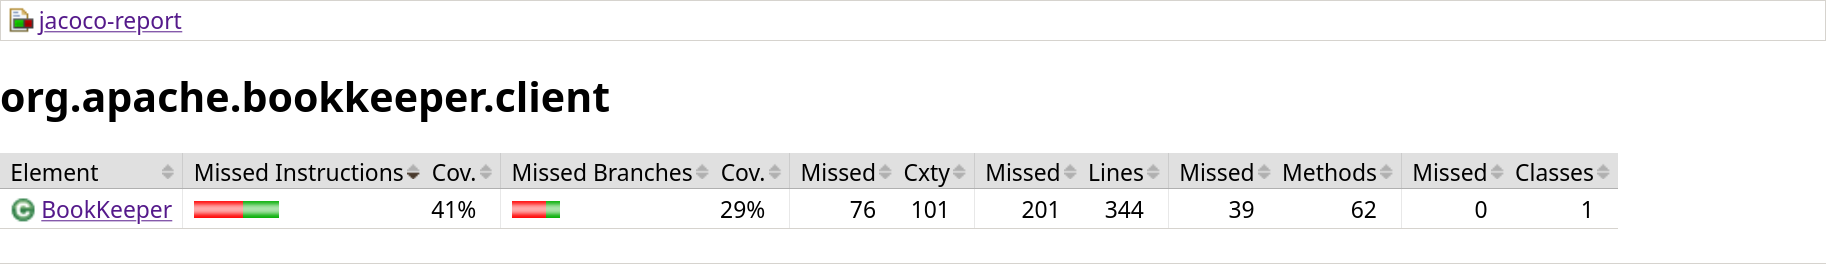
\includegraphics[width=1.0\linewidth, frame]{img/Bookkeeper-before-code-coverage.png}
			\caption{\texttt{Bookkeeper\$Bookkeeper Coverage after Boundary and LLM analysis}}
			\label{fig:BookkeeperCoverage}
		\end{figure}
		
		\begin{figure}
			\centering
			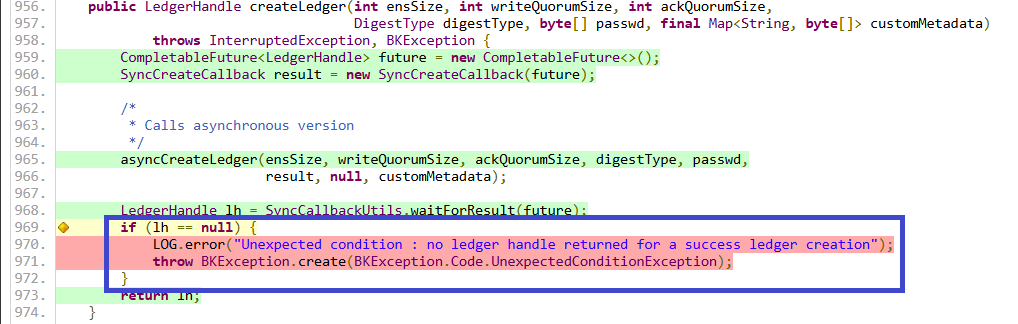
\includegraphics[width=1.0\linewidth, frame]{img/bookkeeper-openledger-branch.png}
			\caption{\texttt{Bookkeeper openLedger}}
			\label{fig:BookkeeperOpenLedger}
		\end{figure}
		
		\begin{figure}
			\centering
			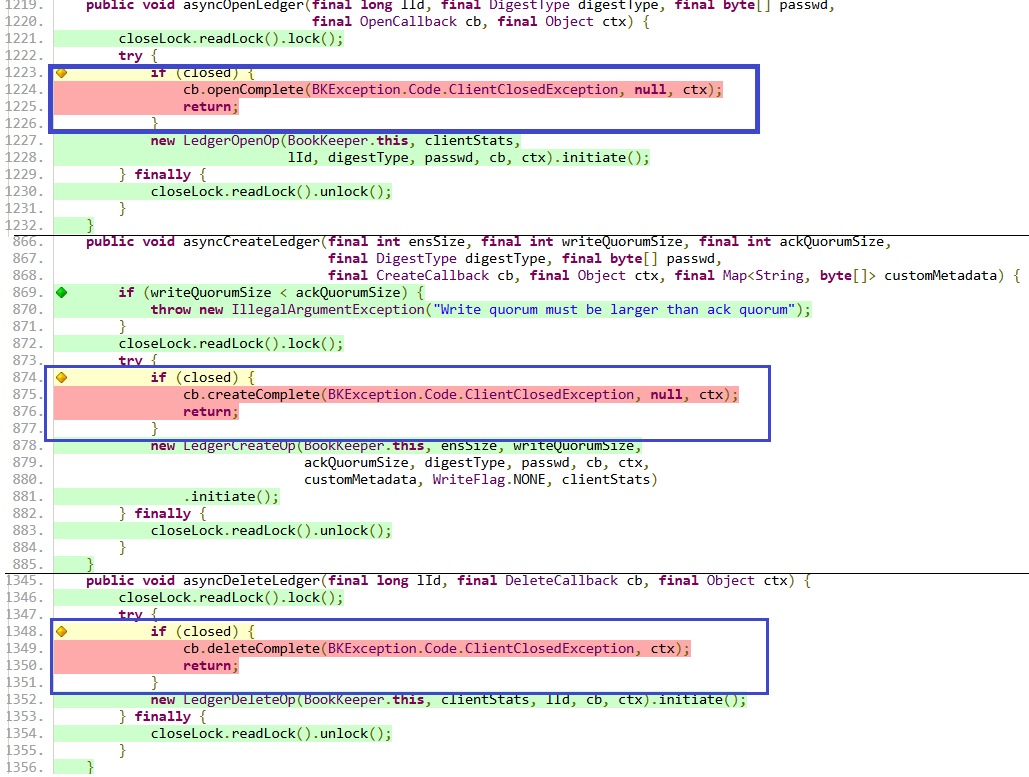
\includegraphics[width=1.0\linewidth, frame]{img/bookkeeper-is_closed-branch.png}
			\caption{\texttt{Bookkeeper isClosed Branch}}
			\label{fig:BookkeeperIsClosed}
		\end{figure}
		
		\begin{figure}
			\centering
			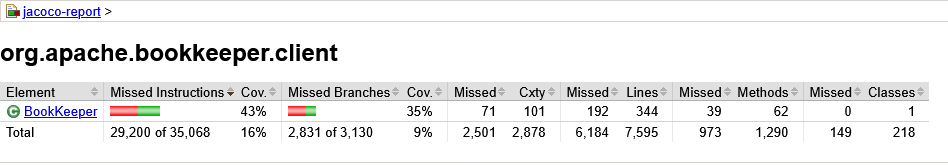
\includegraphics[width=1.0\linewidth, frame]{img/Bookeeper-first-Coverage.png}
			\caption{\texttt{First Branch Coverage}}
			\label{fig:BookeeperFirstCoverage}
		\end{figure}
		
		\begin{figure}
			\centering
			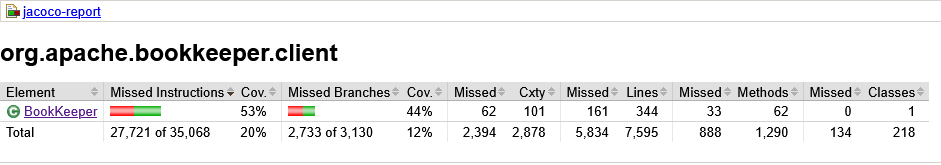
\includegraphics[width=1.0\linewidth, frame]{img/Bookkeeper-last-coverage.png}
			\caption{\texttt{Bookkeeper Final Coverage}}
			\label{fig:BookkeeperLastCoverage}
		\end{figure}
		
		\begin{figure}
			\centering
			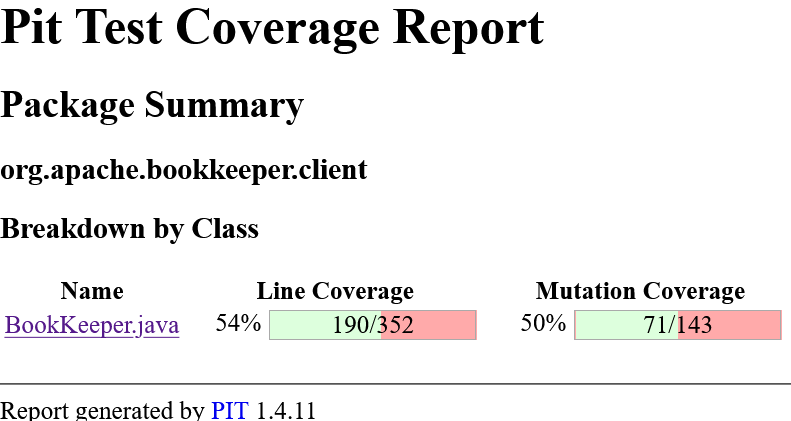
\includegraphics[width=0.5\linewidth, frame]{img/pitest-before-coverage-bk.png}
			\caption{\texttt{Bookkeeper Pitest Before Mutation Coverage}}
			\label{fig:PitestReportBeforeBK}
		\end{figure}
		
		\begin{figure}
			\centering
			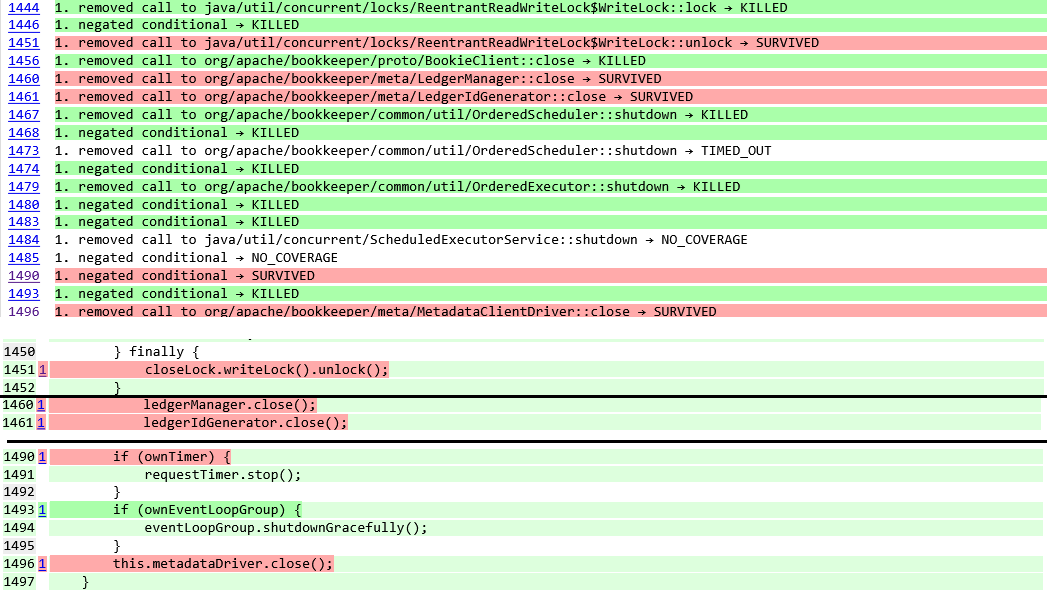
\includegraphics[width=1.0\linewidth, frame]{img/Close-before-mutation-bk.png}
			\caption{\texttt{Bookkeeper.Close Before Mutation Analysis}}
			\label{fig:CloseBeforeMutationBK}
		\end{figure}
		
		\begin{figure}
			\centering
			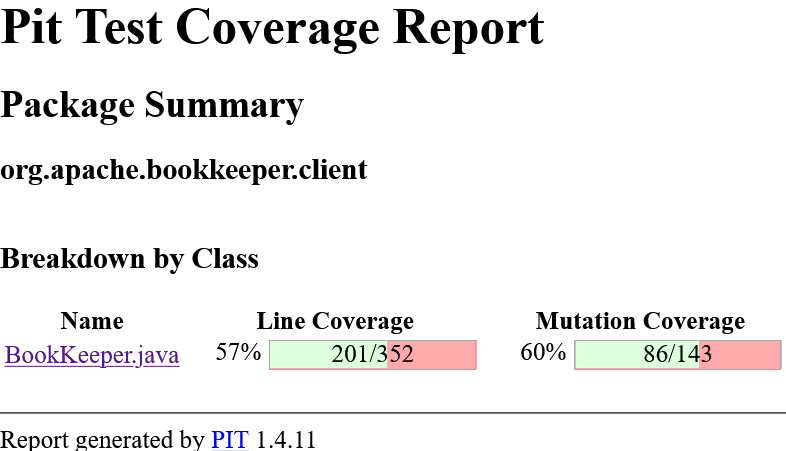
\includegraphics[width=0.5\linewidth, frame]{img/pitest-after-coverage-bk.png}
			\caption{\texttt{Bookkeeper Pitest After Mutation Coverage}}
			\label{fig:PitestReportAfterBK}
		\end{figure}
		
		\begin{figure}
			\centering
			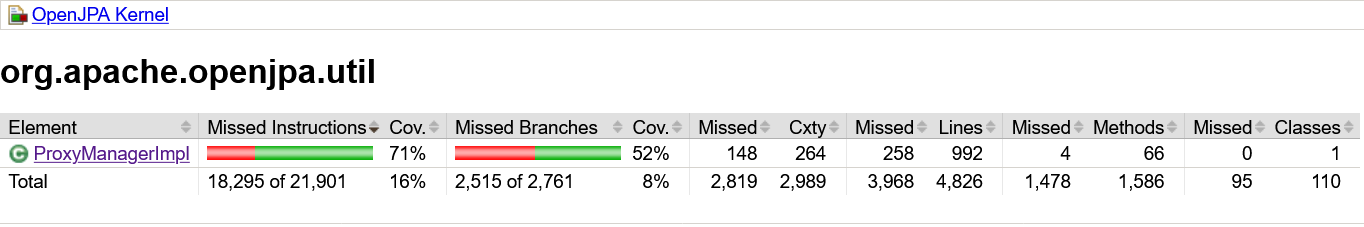
\includegraphics[width=1.0\linewidth, frame]{img/jacoco-report-randoop-ProxyManager.png}
			\caption{\texttt{Coverage JaCoCo Randoop ProxyManagerImpl}}
			\label{fig:JacocoRandoopProxyManagerImpl}
		\end{figure}
		
		\begin{figure}
			\centering
			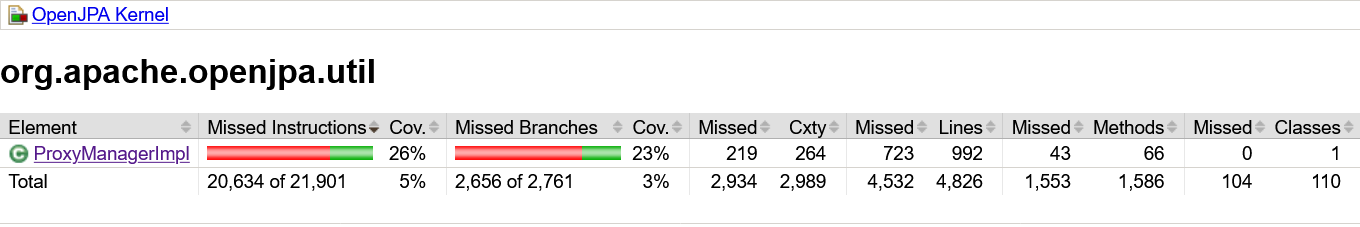
\includegraphics[width=1.0\linewidth, frame]{img/jacoco-report-ba-pm.png}
			\caption{\texttt{Coverage JaCoCo Boundary Analysis}}
			\label{fig:ReportBAPM}
		\end{figure}
		
		\begin{figure}
			\centering
			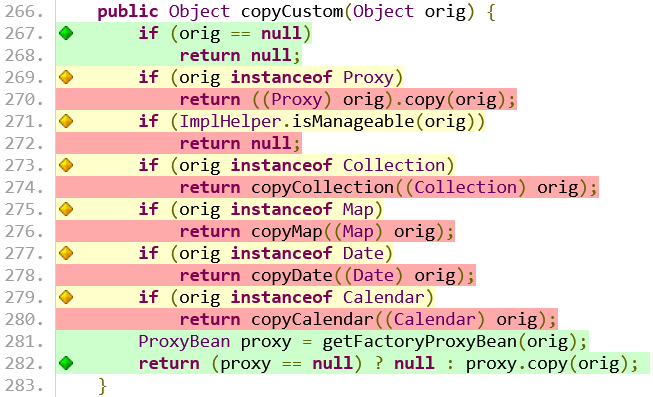
\includegraphics[width=0.5\linewidth, frame]{img/copy-custom.png}
			\caption{\texttt{Coverage JaCoCo Copy Custom}}
			\label{fig:CopyCustom}
		\end{figure}

		
		\section{Tabelle}
		\begin{table}[h]
			\centering
			\begin{tabular}{|c|c|c|c|c|c|c|}
				\hline
				\textbf{es} & \textbf{wQs} & \textbf{aQs} & \textbf{digestType} & \textbf{passwd} & \textbf{customMetaData} & \textbf{atteso} \\
				\hline
				-1 & -2 & -3 & \texttt{DUMMY} & \texttt{byte[]{"password"}} & \texttt{null} & eccezione \\
				\hline
				-1 & -2 & -2 & \texttt{DUMMY} & \texttt{byte[]{"password"}} & \texttt{null} & eccezione \\
				\hline
				-1 & -2 & -1 & \texttt{DUMMY} & \texttt{byte[]{"password"}} & \texttt{null} & eccezione \\
				\hline
				-1 & -1 & -2 & \texttt{DUMMY} & \texttt{byte[]{"password"}} & \texttt{null} & eccezione \\
				\hline
				-1 & -1 & -1 & \texttt{DUMMY} & \texttt{byte[]{"password"}} & \texttt{null} & eccezione \\
				\hline
				-1 & -1 & 0 & \texttt{DUMMY} & \texttt{byte[]{"password"}} & \texttt{null} & eccezione \\
				\hline
				-1 & 0 & -1 & \texttt{DUMMY} & \texttt{byte[]{"password"}} & \texttt{null} & eccezione \\
				\hline
				-1 & 0 & 0 & \texttt{DUMMY} & \texttt{byte[]{"password"}} & \texttt{null} & eccezione \\
				\hline
				-1 & 0 & 1 & \texttt{DUMMY} & \texttt{byte[]{"password"}} & \texttt{null} & eccezione \\
				\hline
				0 & -1 & -2 & \texttt{DUMMY} & \texttt{byte[]{"password"}} & \texttt{null} & valido \\
				\hline
				0 & -1 & -1 & \texttt{DUMMY} & \texttt{byte[]{"password"}} & \texttt{null} & valido \\
				\hline
				0 & -1 & 0 & \texttt{DUMMY} & \texttt{byte[]{"password"}} & \texttt{null} & eccezione \\
				\hline
				0 & 0 & -1 & \texttt{DUMMY} & \texttt{byte[]{"password"}} & \texttt{null} & valido \\
				\hline
				0 & 0 & 0 & \texttt{DUMMY} & \texttt{byte[]{"password"}} & \texttt{null} & valido \\
				\hline
				0 & 0 & 1 & \texttt{DUMMY} & \texttt{byte[]{"password"}} & \texttt{null} & eccezione \\
				\hline
				0 & 1 & 0 & \texttt{DUMMY} & \texttt{byte[]{"password"}} & \texttt{null} & eccezione \\
				\hline
				0 & 1 & 1 & \texttt{DUMMY} & \texttt{byte[]{"password"}} & \texttt{null} & eccezione \\
				\hline
				0 & 1 & 2 & \texttt{DUMMY} & \texttt{byte[]{"password"}} & \texttt{null} & eccezione \\
				\hline
				3 & 2 & 1 & \texttt{DUMMY} & \texttt{byte[]{"password"}} & \texttt{null} & valido \\
				\hline
				3 & 2 & 2 & \texttt{DUMMY} & \texttt{byte[]{"password"}} & \texttt{null} & valido \\
				\hline
				3 & 2 & 3 & \texttt{DUMMY} & \texttt{byte[]{"password"}} & \texttt{null} & eccezione \\
				\hline
				3 & 3 & 2 & \texttt{DUMMY} & \texttt{byte[]{"password"}} & \texttt{null} & valido \\
				\hline
				3 & 3 & 3 & \texttt{DUMMY} & \texttt{byte[]{"password"}} & \texttt{null} & valido \\
				\hline
				3 & 3 & 4 & \texttt{DUMMY} & \texttt{byte[]{"password"}} & \texttt{null} & eccezione \\
				\hline
				3 & 4 & 3 & \texttt{DUMMY} & \texttt{byte[]{"password"}} & \texttt{null} & eccezione \\
				\hline
				3 & 4 & 4 & \texttt{DUMMY} & \texttt{byte[]{"password"}} & \texttt{null} & eccezione \\
				\hline
				3 & 4 & 5 & \texttt{DUMMY} & \texttt{byte[]{"password"}} & \texttt{null} & eccezione \\
				\hline
				4 & 3 & 2 & \texttt{DUMMY} & \texttt{byte[]{"password"}} & \texttt{null} & eccezione \\
				\hline
				4 & 3 & 3 & \texttt{DUMMY} & \texttt{byte[]{"password"}} & \texttt{null} & eccezione \\
				\hline
				4 & 3 & 4 & \texttt{DUMMY} & \texttt{byte[]{"password"}} & \texttt{null} & eccezione \\
				\hline
				4 & 4 & 3 & \texttt{DUMMY} & \texttt{byte[]{"password"}} & \texttt{null} & eccezione \\
				\hline
				4 & 4 & 4 & \texttt{DUMMY} & \texttt{byte[]{"password"}} & \texttt{null} & eccezione \\
				\hline
				4 & 4 & 5 & \texttt{DUMMY} & \texttt{byte[]{"password"}} & \texttt{null} & eccezione \\
				\hline
				4 & 5 & 4 & \texttt{DUMMY} & \texttt{byte[]{"password"}} & \texttt{null} & eccezione \\
				\hline
				4 & 5 & 5 & \texttt{DUMMY} & \texttt{byte[]{"password"}} & \texttt{null} & eccezione \\
				\hline
				4 & 5 & 6 & \texttt{DUMMY} & \texttt{byte[]{"password"}} & \texttt{null} & eccezione \\
				\hline
				3 & 3 & 3 & \texttt{MAC} & \texttt{byte[]{"password"}} & \texttt{null} & valido \\
				\hline
				3 & 3 & 3 & \texttt{CRC32} & \texttt{byte[]{"password"}} & \texttt{null} & valido \\
				\hline
				3 & 3 & 3 & \texttt{CRC32C} & \texttt{byte[]{"password"}} & \texttt{null} & valido \\
				\hline
				3 & 3 & 3 & \texttt{MAC} & \texttt{byte[]{}} & \texttt{null} & valido \\
				\hline
				3 & 3 & 3 & \texttt{MAC} & \texttt{null} & \texttt{null} & eccezione \\
				\hline
				3 & 3 & 3 & \texttt{MAC} & \texttt{byte[]{"password"}} & \texttt{Collection.emptyMap} & valido \\
				\hline
			\end{tabular}
			\caption{Casi di test di \texttt{BookKeeper\#createLedger}. Nota: \texttt{es} = \texttt{ensembleSize}, \texttt{wQs} = \texttt{writeQuorumSize}, \texttt{aQs} = \texttt{ackQuorumSize}}
			\label{tab:test1}
		\end{table}
		
		
		\begin{table}[h]
			\centering
			\resizebox{\textwidth}{!}{
				\begin{tabular}{|c|c|c|c|c|c|c|c|c|}
					\hline
					\textbf{eS} & \textbf{wQs} & \textbf{aQs} & \textbf{digestType} & \textbf{passwd} & \textbf{cb} & \textbf{ctx} & \textbf{customMetaData} & \textbf{atteso} \\
					\hline
					-1 & -2 & -3 & \texttt{DUMMY} & \texttt{byte[]{"password"}} & \texttt{SyncCreateCallback} & \texttt{"TEST CTX"} & \texttt{null} & eccezione \\
					\hline
					-1 & -2 & -2 & \texttt{DUMMY} & \texttt{byte[]{"password"}} & \texttt{SyncCreateCallback} & \texttt{"TEST CTX"} & \texttt{null} & eccezione \\
					\hline
					-1 & -2 & -1 & \texttt{DUMMY} & \texttt{byte[]{"password"}} & \texttt{SyncCreateCallback} & \texttt{"TEST CTX"} & \texttt{null} & eccezione \\
					\hline
					-1 & -1 & -2 & \texttt{DUMMY} & \texttt{byte[]{"password"}} & \texttt{SyncCreateCallback} & \texttt{"TEST CTX"} & \texttt{null} & eccezione \\
					\hline
					-1 & -1 & -1 & \texttt{DUMMY} & \texttt{byte[]{"password"}} & \texttt{SyncCreateCallback} & \texttt{"TEST CTX"} & \texttt{null} & eccezione \\
					\hline
					-1 & -1 & 0 & \texttt{DUMMY} & \texttt{byte[]{"password"}} & \texttt{SyncCreateCallback} & \texttt{"TEST CTX"} & \texttt{null} & eccezione \\
					\hline
					-1 & 0 & -1 & \texttt{DUMMY} & \texttt{byte[]{"password"}} & \texttt{SyncCreateCallback} & \texttt{"TEST CTX"} & \texttt{null} & eccezione \\
					\hline
					-1 & 0 & 0 & \texttt{DUMMY} & \texttt{byte[]{"password"}} & \texttt{SyncCreateCallback} & \texttt{"TEST CTX"} & \texttt{null} & eccezione \\
					\hline
					-1 & 0 & 1 & \texttt{DUMMY} & \texttt{byte[]{"password"}} & \texttt{SyncCreateCallback} & \texttt{"TEST CTX"} & \texttt{null} & eccezione \\
					\hline
					0 & -1 & -2 & \texttt{DUMMY} & \texttt{byte[]{"password"}} & \texttt{SyncCreateCallback} & \texttt{"TEST CTX"} & \texttt{null} & valido \\
					\hline
					0 & -1 & -1 & \texttt{DUMMY} & \texttt{byte[]{"password"}} & \texttt{SyncCreateCallback} & \texttt{"TEST CTX"} & \texttt{null} & valido \\
					\hline
					0 & -1 & 0 & \texttt{DUMMY} & \texttt{byte[]{"password"}} & \texttt{SyncCreateCallback} & \texttt{"TEST CTX"} & \texttt{null} & eccezione \\
					\hline
					0 & 0 & -1 & \texttt{DUMMY} & \texttt{byte[]{"password"}} & \texttt{SyncCreateCallback} & \texttt{"TEST CTX"} & \texttt{null} & valido \\
					\hline
					0 & 0 & 0 & \texttt{DUMMY} & \texttt{byte[]{"password"}} & \texttt{SyncCreateCallback} & \texttt{"TEST CTX"} & \texttt{null} & valido \\
					\hline
					0 & 0 & 1 & \texttt{DUMMY} & \texttt{byte[]{"password"}} & \texttt{SyncCreateCallback} & \texttt{"TEST CTX"} & \texttt{null} & eccezione \\
					\hline
					0 & 1 & 0 & \texttt{DUMMY} & \texttt{byte[]{"password"}} & \texttt{SyncCreateCallback} & \texttt{"TEST CTX"} & \texttt{null} & eccezione \\
					\hline
					0 & 1 & 1 & \texttt{DUMMY} & \texttt{byte[]{"password"}} & \texttt{SyncCreateCallback} & \texttt{"TEST CTX"} & \texttt{null} & eccezione \\
					\hline
					0 & 1 & 2 & \texttt{DUMMY} & \texttt{byte[]{"password"}} & \texttt{SyncCreateCallback} & \texttt{"TEST CTX"} & \texttt{null} & eccezione \\
					\hline
					3 & 2 & 1 & \texttt{DUMMY} & \texttt{byte[]{"password"}} & \texttt{SyncCreateCallback} & \texttt{"TEST CTX"} & \texttt{null} & valido \\
					\hline
					3 & 2 & 2 & \texttt{DUMMY} & \texttt{byte[]{"password"}} & \texttt{SyncCreateCallback} & \texttt{"TEST CTX"} & \texttt{null} & valido \\
					\hline
					3 & 2 & 3 & \texttt{DUMMY} & \texttt{byte[]{"password"}} & \texttt{SyncCreateCallback} & \texttt{"TEST CTX"} & \texttt{null} & eccezione \\
					\hline
					3 & 3 & 2 & \texttt{DUMMY} & \texttt{byte[]{"password"}} & \texttt{SyncCreateCallback} & \texttt{"TEST CTX"} & \texttt{null} & valido \\
					\hline
					3 & 3 & 3 & \texttt{DUMMY} & \texttt{byte[]{"password"}} & \texttt{SyncCreateCallback} & \texttt{"TEST CTX"} & \texttt{null} & valido \\
					\hline
					3 & 3 & 4 & \texttt{DUMMY} & \texttt{byte[]{"password"}} & \texttt{SyncCreateCallback} & \texttt{"TEST CTX"} & \texttt{null} & eccezione \\
					\hline
					3 & 4 & 3 & \texttt{DUMMY} & \texttt{byte[]{"password"}} & \texttt{SyncCreateCallback} & \texttt{"TEST CTX"} & \texttt{null} & eccezione \\
					\hline
					3 & 4 & 4 & \texttt{DUMMY} & \texttt{byte[]{"password"}} & \texttt{SyncCreateCallback} & \texttt{"TEST CTX"} & \texttt{null} & eccezione \\
					\hline
					3 & 4 & 5 & \texttt{DUMMY} & \texttt{byte[]{"password"}} & \texttt{SyncCreateCallback} & \texttt{"TEST CTX"} & \texttt{null} & eccezione \\
					\hline
					4 & 3 & 2 & \texttt{DUMMY} & \texttt{byte[]{"password"}} & \texttt{SyncCreateCallback} & \texttt{"TEST CTX"} & \texttt{null} & eccezione \\
					\hline
					4 & 3 & 3 & \texttt{DUMMY} & \texttt{byte[]{"password"}} & \texttt{SyncCreateCallback} & \texttt{"TEST CTX"} & \texttt{null} & eccezione \\
					\hline
					4 & 3 & 4 & \texttt{DUMMY} & \texttt{byte[]{"password"}} & \texttt{SyncCreateCallback} & \texttt{"TEST CTX"} & \texttt{null} & eccezione \\
					\hline
					4 & 4 & 3 & \texttt{DUMMY} & \texttt{byte[]{"password"}} & \texttt{SyncCreateCallback} & \texttt{"TEST CTX"} & \texttt{null} & eccezione \\
					\hline
					4 & 4 & 4 & \texttt{DUMMY} & \texttt{byte[]{"password"}} & \texttt{SyncCreateCallback} & \texttt{"TEST CTX"} & \texttt{null} & eccezione \\
					\hline
					4 & 4 & 5 & \texttt{DUMMY} & \texttt{byte[]{"password"}} & \texttt{SyncCreateCallback} & \texttt{"TEST CTX"} & \texttt{null} & eccezione \\
					\hline
					4 & 5 & 4 & \texttt{DUMMY} & \texttt{byte[]{"password"}} & \texttt{SyncCreateCallback} & \texttt{"TEST CTX"} & \texttt{null} & eccezione \\
					\hline
					4 & 5 & 5 & \texttt{DUMMY} & \texttt{byte[]{"password"}} & \texttt{SyncCreateCallback} & \texttt{"TEST CTX"} & \texttt{null} & eccezione \\
					\hline
					4 & 5 & 6 & \texttt{DUMMY} & \texttt{byte[]{"password"}} & \texttt{SyncCreateCallback} & \texttt{"TEST CTX"} & \texttt{null} & eccezione \\
					\hline
					3 & 3 & 3 & \texttt{MAC} & \texttt{byte[]{"password"}} & \texttt{SyncCreateCallback} & \texttt{"TEST CTX"} & \texttt{null} & valido \\
					\hline
					3 & 3 & 3 & \texttt{CRC32} & \texttt{byte[]{"password"}} & \texttt{SyncCreateCallback} & \texttt{"TEST CTX"} & \texttt{null} & valido \\
					\hline
					3 & 3 & 3 & \texttt{CRC32C} & \texttt{byte[]{"password"}} & \texttt{SyncCreateCallback} & \texttt{"TEST CTX"} & \texttt{null} & valido \\
					\hline
					3 & 3 & 3 & \texttt{MAC} & \texttt{byte[]{}} & \texttt{SyncCreateCallback} & \texttt{"TEST CTX"} & \texttt{null} & valido \\
					\hline
					3 & 3 & 3 & \texttt{MAC} & \texttt{null} & \texttt{SyncCreateCallback} & \texttt{"TEST CTX"} & \texttt{null} & eccezione \\
					\hline
					3 & 3 & 3 & \texttt{MAC} & \texttt{byte[]{"password"}} & \texttt{SyncCreateCallback} & \texttt{"TEST CTX"} & \texttt{Collection.emptyMap} & valido \\
					\hline
					3 & 3 & 3 & \texttt{MAC} & \texttt{byte[]{"password"}} & \texttt{null} & \texttt{"TEST CTX"} & \texttt{Collection.emptyMap} & eccezione \\
					\hline
					3 & 3 & 3 & \texttt{MAC} & \texttt{byte[]{"password"}} & \texttt{IvalidSyncCreateCb} & \texttt{"TEST CTX"} & \texttt{Collection.emptyMap} & eccezione \\
					\hline
					3 & 3 & 3 & \texttt{MAC} & \texttt{byte[]{"password"}} & \texttt{SyncCreateCallback} & \texttt{null} & \texttt{Collection.emptyMap} & valido \\
					\hline
				\end{tabular}
			}
			\caption{Casi di test di \texttt{BookKeeper\#asyncCreateLedger}}
			\label{tab:test2}
		\end{table}
		
		
		\begin{table}[h]
			\centering
			\begin{tabular}{|c|c|c|c|}
				\hline
				\textbf{lld} & \textbf{digestType} & \textbf{passwd} & \textbf{atteso} \\
				\hline
				-1 & \texttt{DUMMY} & \texttt{byte[]{"Valid Password"}} & eccezione \\
				\hline
				0 & \texttt{DUMMY} & \texttt{byte[]{"Valid Password"}} & valido \\
				\hline
				0 & \texttt{MAC} & \texttt{byte[]{"Valid Password"}} & valido \\
				\hline
				0 & \texttt{CRC32} & \texttt{byte[]{"Valid Password"}} & valido \\
				\hline
				0 & \texttt{CRC32C} & \texttt{byte[]{"Valid Password"}} & valido \\
				\hline
				0 & \texttt{CRC32C} & \texttt{byte[]{"Invalid Password"}} & eccezione \\
				\hline
				0 & \texttt{CRC32C} & \texttt{null} & eccezione \\
				\hline
				0 & \texttt{CRC32C} & \texttt{byte[]{}} & eccezione \\
				\hline
				1 & \texttt{CRC32C} & \texttt{byte[]{"Valid Password"}} & eccezione \\
				\hline
			\end{tabular}
			\caption{Casi di test di \texttt{BookKeeper\#openLedger}}
			\label{tab:test3}
		\end{table}
		
		
		\begin{table}[h]
			\centering
			\begin{tabular}{|c|c|c|c|c|c|}
				\hline
				\textbf{lld} & \textbf{digestType} & \textbf{passwd} & \textbf{cb} & \textbf{ctx} & \textbf{atteso} \\
				\hline
				-1 & \texttt{DUMMY} & \texttt{byte[]{"Valid Password"}} & \texttt{SyncOpenCallback} & \texttt{"TESTS OPEN CTX"} & eccezione \\
				\hline
				0 & \texttt{DUMMY} & \texttt{byte[]{"Valid Password"}} & \texttt{SyncOpenCallback} & \texttt{"TESTS OPEN CTX"} & valido \\
				\hline
				0 & \texttt{MAC} & \texttt{byte[]{"Valid Password"}} & \texttt{SyncOpenCallback} & \texttt{"TESTS OPEN CTX"} & valido \\
				\hline
				0 & \texttt{CRC32} & \texttt{byte[]{"Valid Password"}} & \texttt{SyncOpenCallback} & \texttt{"TESTS OPEN CTX"} & valido \\
				\hline
				0 & \texttt{CRC32C} & \texttt{byte[]{"Valid Password"}} & \texttt{SyncOpenCallback} & \texttt{"TESTS OPEN CTX"} & valido \\
				\hline
				0 & \texttt{CRC32C} & \texttt{byte[]{"Invalid Password"}} & \texttt{SyncOpenCallback} & \texttt{"TESTS OPEN CTX"} & eccezione \\
				\hline
				0 & \texttt{CRC32C} & \texttt{null} & \texttt{SyncOpenCallback} & \texttt{"TESTS OPEN CTX"} & eccezione \\
				\hline
				0 & \texttt{CRC32C} & \texttt{byte[]{}} & \texttt{SyncOpenCallback} & \texttt{"TESTS OPEN CTX"} & eccezione \\
				\hline
				1 & \texttt{CRC32C} & \texttt{byte[]{"Valid Password"}} & \texttt{SyncOpenCallback} & \texttt{"TESTS OPEN CTX"} & eccezione \\
				\hline
				0 & \texttt{MAC} & \texttt{byte[]{"Valid Password"}} & \texttt{InvalidOpenCallback} & \texttt{"TESTS OPEN CTX"} & eccezione \\
				\hline
				0 & \texttt{MAC} & \texttt{byte[]{"Valid Password"}} & \texttt{null} & \texttt{"TESTS OPEN CTX"} & eccezione \\
				\hline
				0 & \texttt{MAC} & \texttt{byte[]{"Valid Password"}} & \texttt{SyncOpenCallback} & \texttt{null} & valido \\
				\hline
			\end{tabular}
			\caption{Casi di test di \texttt{BookKeeper\#asyncOpenLedger}}
			\label{tab:test4}
		\end{table}
		
		\begin{table}[h]
			\centering
			\begin{tabular}{|c|c|c|c|c|c|}
				\hline
				\textbf{data} & \textbf{offset} & \textbf{length} & \textbf{cb} & \textbf{ctx} & \textbf{atteso} \\
				\hline
				\texttt{null} & 0 & -1 & \texttt{new SyncAddCallback()} & \texttt{"ctx"} & \texttt{ArrayIndexOutOfBoundsException} \\
				\hline
				\texttt{null} & 0 & 0 & \texttt{new SyncAddCallback()} & \texttt{"ctx"} & \texttt{NullPointerException} \\
				\hline
				\texttt{null} & 0 & 1 & \texttt{new SyncAddCallback()} & \texttt{"ctx"} & \texttt{NullPointerException} \\
				\hline
				\texttt{Byte[]\{\}} & 0 & -1 & \texttt{new SyncAddCallback()} & \texttt{"ctx"} & \texttt{ArrayIndexOutOfBoundsException} \\
				\hline
				\texttt{Byte[]\{\}} & 0 & 0 & \texttt{new SyncAddCallback()} & \texttt{"ctx"} & \texttt{Valido} \\
				\hline
				\texttt{Byte[]\{\}} & 0 & 1 & \texttt{new SyncAddCallback()} & \texttt{"ctx"} & \texttt{ArrayIndexOutOfBoundsException} \\
				\hline
				\texttt{Byte[]{"test"}} & 0 & 3 & \texttt{new SyncAddCallback()} & \texttt{"ctx"} & \texttt{Valido} \\
				\hline
				\texttt{Byte[]{"test"}} & 0 & 4 & \texttt{new SyncAddCallback()} & \texttt{"ctx"} & \texttt{Valido} \\
				\hline
				\texttt{Byte[]{"test"}} & 0 & 5 & \texttt{new SyncAddCallback()} & \texttt{"ctx"} & \texttt{ArrayIndexOutOfBoundsException} \\
				\hline
				\texttt{Byte[]{"test"}} & 0 & 4 & \texttt{new InvalAddCallback()} & \texttt{"ctx"} & \texttt{BKException.Code.IllegalOpException} \\
				\hline
				\texttt{Byte[]{"test"}} & 0 & 4 & \texttt{null} & \texttt{"ctx"} & \texttt{NullPointerException} \\
				\hline
				\texttt{Byte[]{"test"}} & 0 & 4 & \texttt{new SyncAddCallback()} & \texttt{null} & \texttt{Valido} \\
				\hline
				\texttt{Byte[]{"test"}} & 1 & 4 & \texttt{new SyncAddCallback()} & \texttt{"ctx"} & \texttt{ArrayIndexOutOfBoundsException} \\
				\hline
				\texttt{Byte[]{"test"}} & -1 & 4 & \texttt{new SyncAddCallback()} & \texttt{"ctx"} & \texttt{ArrayIndexOutOfBoundsException} \\
				\hline
			\end{tabular}
			\caption{Casi di test di \texttt{LedgerHandle\#asyncAddEntry}}
			\label{tab:addEntryLedger}
		\end{table}
		
		
		\begin{table}[h]
			\centering
			\begin{tabular}{|c|c|c|c|c|}
				\hline
				\textbf{firstEntry} & \textbf{lastEntry} & \textbf{cb} & \textbf{ctx} & \textbf{atteso} \\
				\hline
				-1 & -2 & \texttt{new SyncReadCallback()} & \texttt{"ctx"} & \texttt{BKException.Code.IncorrectParameterException} \\
				\hline
				-1 & -1 & \texttt{new SyncReadCallback()} & \texttt{"ctx"} & \texttt{BKException.Code.IncorrectParameterException} \\
				\hline
				-1 & 2 & \texttt{new SyncReadCallback()} & \texttt{"ctx"} & \texttt{BKException.Code.IncorrectParameterException} \\
				\hline
				0 & -1 & \texttt{new SyncReadCallback()} & \texttt{"ctx"} & 
				\texttt{BKException.Code.IncorrectParameterException} \\
				\hline
				0 & 0 & \texttt{new SyncReadCallback()} & \texttt{"ctx"} & \texttt{Valido} \\
				\hline
				0 & 2 & \texttt{new SyncReadCallback()} & \texttt{"ctx"} & \texttt{Valido} \\
				\hline
				2 & 1 & \texttt{new SyncReadCallback()} & \texttt{"ctx"} & \texttt{BKException.Code.IncorrectParameterException} \\
				\hline
				2 & 2 & \texttt{new SyncReadCallback()} & \texttt{"ctx"} & \texttt{Valido} \\
				\hline
				2 & 3 & \texttt{new SyncReadCallback()} & \texttt{"ctx"} & \texttt{BKException.Code.BKReadException} \\
				\hline
				3 & 2 & \texttt{new SyncReadCallback()} & \texttt{"ctx"} & \texttt{BKException.Code.IncorrectParameterException} \\
				\hline
				3 & 3 & \texttt{new SyncReadCallback()} & \texttt{"ctx"} & \texttt{BKException.Code.BKReadException} \\
				\hline
				3 & 4 & \texttt{new SyncReadCallback()} & \texttt{"ctx"} & \texttt{BKException.Code.BKReadException} \\
				\hline
				0 & 2 & \texttt{new InvalidReadCallback()} & \texttt{"ctx"} & \texttt{BKException.Code.IllegalOpException} \\
				\hline
				0 & 2 & \texttt{new SyncReadCallback()} & \texttt{null} & \texttt{Valido} \\
				\hline
				0 & 2 & \texttt{new SyncReadCallback()} & \texttt{null} & \texttt{Valido} \\
				\hline
				
			\end{tabular}
			\caption{Casi di test di \texttt{LedgerHandle\#readEntries}}
			\label{tab:readEntriesLedger}
		\end{table}
		
		
		\begin{table}[h]
			\centering
			\begin{tabular}{|c|c|}
				\hline
				\textbf{orig} & \textbf{atteso} \\
				\hline
				\texttt{AValidProxy} & Copia dell'istanza \\
				\hline
				\texttt{AnInvalidProxy} & \texttt{null} \\
				\hline
				\texttt{null} & \texttt{null} \\
				\hline
			\end{tabular}
			\caption{Casi di test di \texttt{OpenJPA\#copyCustom}}
			\label{tab:test5}
		\end{table}
		
		
		\begin{table}[h]
			\centering
			\begin{tabular}{|c|c|c|}
				\hline
				\textbf{orig} & \textbf{autoOff} & \textbf{atteso} \\
				\hline
				\texttt{AValidProxy} & \texttt{false} & Proxy dell'istanza \\
				\hline
				\texttt{AValidProxy} & \texttt{true} & Proxy dell'istanza \\
				\hline
				\texttt{AnInvalidProxy} & \texttt{false} & \texttt{null} \\
				\hline
				\texttt{null} & \texttt{false} & \texttt{null} \\
				\hline
			\end{tabular}
			\caption{Casi di test di \texttt{OpenJPA\#newCustomProxy}}
			\label{tab:test5}
		\end{table}
		
		
		\begin{table}[h]
			\centering
			\begin{tabular}{|l|c|l|}
				\hline
				\textbf{Caso} & \textbf{orig} & \textbf{Risultato atteso} \\
				\hline
				CC1 & null & null \\
				\hline
				CC2 & AValidProxy (implementa Proxy) & Copia tramite \texttt{Proxy.copy(orig)} \\
				\hline
				CC3 & ManageableEntity (gestibile) & null \\
				\hline
				CC4 & ArrayList\textless{}\texttt{String}\textgreater{} & Copia della collection \\
				\hline
				CC5 & HashMap\textless{}\texttt{K,V}\textgreater{} & Copia della mappa \\
				\hline
				CC6 & Date & Copia della data \\
				\hline
				CC7 & Calendar.getInstance() & Copia del calendario \\
				\hline
				CC8 & Bean con ProxyBean valido & Copia tramite \texttt{proxy.copy(orig)} \\
				\hline
				CC9 & Bean con ProxyBean nullo & null \\
				\hline
				CC10 & Oggetto non gestibile/non proxyable (fallback) & null \\
				\hline
			\end{tabular}
			\caption{Casi MC/DC per il metodo \texttt{copyCustom(Object orig)}}
			\label{tab:mcdc_copycustom}
		\end{table}
		
		
		\begin{table}[h]
			\centering
			\begin{tabular}{|l|c|c|l|}
				\hline
				\textbf{Caso} & \textbf{orig} & \textbf{autoOff} & \textbf{Risultato atteso} \\
				\hline
				NC1 & null & - & null \\
				\hline
				NC2 & AValidProxy (implementa Proxy) & - & Stessa istanza restituita \\
				\hline
				NC3 & ManageableEntity (gestibile) & - & null \\
				\hline
				NC4 & Bean non proxyable & - & null \\
				\hline
				NC5 & ArrayList\textless{}\texttt{String}\textgreater{} & false & Proxy della collection \\
				\hline
				NC6 & ArrayList\textless{}\texttt{String}\textgreater{} & true & Proxy della collection (autoOff) \\
				\hline
				NC7 & HashMap\textless{}\texttt{K,V}\textgreater{} & false & Proxy della mappa \\
				\hline
				NC8 & Date & - & Proxy della data \\
				\hline
				NC9 & Calendar.getInstance() & - & Proxy del calendario \\
				\hline
				NC10 & Bean con ProxyBean valido & - & Istanza proxy da \texttt{proxy.newInstance(orig)} \\
				\hline
				NC11 & Bean con ProxyBean nullo & - & null \\
				\hline
			\end{tabular}
			\caption{Casi MC/DC per il metodo \texttt{newCustomProxy(Object orig, boolean autoOff)}}
			\label{tab:mcdc_newcustomproxy}
		\end{table}
		
	\end{document}
	
